\documentclass[12pt]{article}

\usepackage{amsmath}
\usepackage{amssymb}
\usepackage{amsthm}
\usepackage{etoolbox}
\usepackage{hyperref}
\usepackage{geometry}
\usepackage{booktabs}
\usepackage{draftwatermark}
\SetWatermarkText{DRAFT}
\SetWatermarkScale{1.5}
\SetWatermarkColor[gray]{0.85}

\geometry{margin=1in}

%------------------------------------------------------------
% Theorem environments
%------------------------------------------------------------
\newtheorem{theorem}{Theorem}[section]
\newtheorem{lemma}[theorem]{Lemma}
\newtheorem{proposition}[theorem]{Proposition}
\newtheorem{corollary}[theorem]{Corollary}
\theoremstyle{definition}
\newtheorem{definition}[theorem]{Definition}
\newtheorem{example}[theorem]{Example}
\theoremstyle{remark}
\newtheorem{remark}[theorem]{Remark}
\theoremstyle{plain}
\newtheorem{conjecture}[theorem]{Conjecture}

% Add selected theorem-like environments to the TOC.
% Patch amsthm's \@begintheorem{Name}{Number}[Title] to emit a TOC entry
% for Theorem, Lemma, Definition, Corollary, and Proposition.
\makeatletter
\let\thmt@orig@begintheorem\@begintheorem
\def\thmt@addtotoc#1#2#3{%
  % #1 = env name, #2 = number, #3 = optional title (may be empty)
  \def\thmt@do##1{%
    \edef\thmt@cur{##1}%
    \edef\thmt@name{#1}%
    \ifx\thmt@cur\thmt@name
      \def\thmt@title{#3}%
      \ifx\thmt@title\@empty
        \addcontentsline{toc}{subsubsection}{#1~#2}%
      \else
        \addcontentsline{toc}{subsubsection}{#1~#2\space(#3)}%
      \fi
    \fi
  }%
  \thmt@do{Theorem}%
  \thmt@do{Lemma}%
  \thmt@do{Definition}%
  \thmt@do{Corollary}%
  \thmt@do{Proposition}%
}
\def\@begintheorem#1#2[#3]{%
  \thmt@addtotoc{#1}{#2}{#3}%
  \thmt@orig@begintheorem{#1}{#2}[#3]%
}
\makeatother

%------------------------------------------------------------
% Notation macros
%------------------------------------------------------------
\newcommand{\ZZ}{\mathbb{Z}}
\newcommand{\NN}{\mathbb{N}}
\newcommand{\RR}{\mathbb{R}}
\newcommand{\lam}{\lambda}
\newcommand{\eps}{\varepsilon}
\newcommand{\OO}{\mathsf{O}}
\newcommand{\EE}{\mathsf{E}}
\newcommand{\Kval}{K}
\newcommand{\Dval}{\Delta}
\newcommand{\tgt}{\theta}
\newcommand{\wplus}{w^{+}}
\newcommand{\wminus}{w^{-}}
\newcommand{\rplus}{r_{+}}
\newcommand{\rminus}{r_{-}}
\newcommand{\eplus}{e_{+}}
\newcommand{\eminus}{e_{-}}
\newcommand{\odenp}{o_{+}}
\newcommand{\odenm}{o_{-}}
\newcommand{\epsplus}{\eps_{+}}
\newcommand{\epsminus}{\eps_{-}}
\newcommand{\lamplus}{\lam_{+}}
\newcommand{\lamminus}{\lam_{-}}

%------------------------------------------------------------
\title{Mediant Trees for Rational Approximation and Sturmian Word Generation}
\author{Jon Seymour}
\date{\today}
%------------------------------------------------------------

\begin{document}

\maketitle

\begin{abstract}
Given an oracle for a real number $\theta$ of sufficient precision, we present four
contributions.
First, an algorithm that constructs a \emph{mediant tree} of increasingly precise rational
approximations to $\theta$: starting from a Farey-adjacent bounded pair bracketing $\theta$,
each iteration applies a weighted mediant step with an optimal integer weight $\wplus$ given by
a closed-form formula (Theorem~\ref{thm:optimal-w}).
The denominator structure mirrors the classical continued-fraction recurrence
(Section~\ref{sec:convergence}), though a proof of superlinear growth remains open.
Second, a Sturmian transduction that converts the mediant tree into a \emph{mediant word}
--- a string over $\{\OO, \EE\}$ encoding the full approximation path --- and establishes
that this word is identical to the Sturmian word with slope $1/(1+\theta)$ at all interior
positions, with the terminal symbol of each finite prefix fully characterised by whether
$r$ is an overestimate or underestimate of $\theta$ (Theorem~\ref{prop:sturmian}).
Third, we prove two structural invariants of mediant words: every non-leaf word begins
with $\EE\EE$ (Theorem~\ref{prop:EE-prefix}), and the interior slice
$\pi(r)[1{:}L{-}1]$ of any mediant word of length $L \geq 2$ is a palindrome
(Theorem~\ref{prop:palindrome}).
Fourth, we show how to extend both algorithms to real numbers $\theta \in (0, 1)$ and
$\theta < 0$ via simple algebraic reductions to the $\theta > 1$ case.
\end{abstract}

\tableofcontents

%------------------------------------------------------------
\section{Introduction}
\label{sec:intro}
%------------------------------------------------------------

The approximation of irrational numbers by rationals is a classical subject in number theory.
The Stern--Brocot tree and Farey sequences provide a systematic account of best rational
approximants, and the continued-fraction expansion of a real number yields its
convergents --- the fractions closest to the target with bounded denominator.
Sturmian words, introduced by Morse and Hedlund~\cite{morse1940}, give a
combinatorial counterpart: the infinite binary sequence $s_n = \lfloor(n+1)\alpha\rfloor -
\lfloor n\alpha\rfloor$ with slope $\alpha \in (0,1)$ is the unique balanced aperiodic
sequence with $\mathsf{O}$-density $\alpha$.

The present paper makes four contributions to this classical picture.
\begin{enumerate}
  \item \textbf{Optimal weight formula.}
    We introduce the \emph{bounded-pair} framework, in which two Farey-adjacent rational
    estimates bracket $\theta$ from above and below.
    Each weighted mediant step is a run of $w$ steps in the Stern--Brocot tree in the
    same direction --- the classical construction (see Graham, Knuth and
    Patashnik~\cite{gkp1994}).
    What is new is Theorem~\ref{thm:optimal-w}: a closed-form expression for the unique
    \emph{optimal} integer weight $\wplus$ --- the one whose mediants straddle $\theta$
    --- derived from a sign-change bracket on the linear error function, enabling
    efficient iteration with no redundant steps.
  \item \textbf{Mediant word representation.}
    The mediant tree can be encoded as a string over $\{\OO, \EE\}$, the
    \emph{mediant word} (Section~\ref{sec:parity}).
    This representation connects rational approximation to combinatorics on words.
  \item \textbf{Sturmian identity.}
    The mediant word produced by the mediant tree is identical to the
    Sturmian word with slope $1/(1+\theta)$
    (Theorem~\ref{prop:sturmian}), agreeing at every position except possibly the last
    symbol of each finite prefix.
    The identification of Christoffel words with Sturmian prefixes is classical
    (Lothaire~\cite{lothaire2002}); the novelty is the direct proof via the mediant
    construction and the precise last-letter criterion.
  \item \textbf{Compressed transducer.}
    Each iterate produced by the algorithm is at least a Stern--Brocot semi-convergent --- the
    best bracketing fraction achievable in one step from the current bounded pair.
    The mediant tree is therefore a \emph{compressed transducer} for the Sturmian word:
    the approximation path (empirically $O(\log N)$ integer-arithmetic steps; a formal
    bound remains open) encodes the entire construction history, after which the $N$
    symbols are enumerated by a purely integer recursive traversal with no further
    real arithmetic.
\end{enumerate}

The algorithm requires an oracle for $\theta$ --- a means of evaluating
$\lceil o\theta \rceil$ to sufficient precision at each step --- but is otherwise entirely
general.
Given such an oracle, the mediant tree can represent \emph{any} real number as a mediant
word over $\{\OO, \EE\}$, making it a universal encoder from reals to binary words.

\paragraph{Organisation.}
Part~I (Sections~\ref{sec:background-sb}--\ref{sec:background-deluca}) collects
background on the Stern--Brocot tree, Farey sequences, Sturmian words, and Christoffel
words.
Part~II develops the algorithm and its theory:
Section~\ref{sec:definitions} introduces the core definitions;
Section~\ref{sec:mediant} develops the mediant construction and straddling inequality;
Section~\ref{sec:optimal-w} derives the optimal weight formula;
Section~\ref{sec:parity} introduces mediant words;
Section~\ref{sec:tree} describes the mediant tree;
Section~\ref{sec:convergence} analyses the rate of convergence;
Section~\ref{sec:examples} presents examples and computational results;
Section~\ref{sec:sturmian} establishes the connection to Sturmian words;
Section~\ref{sec:extension} extends the construction to all real $\theta \notin \{0,1\}$;
Section~\ref{sec:conclusion} concludes with open questions.
Appendix~\ref{app:optimal-w} contains the proof of Theorem~\ref{thm:optimal-w}.

%============================================================
\part{Background}
%============================================================

%------------------------------------------------------------
\section{The Stern--Brocot Tree and Mediants}
\label{sec:background-sb}
%------------------------------------------------------------

The \emph{Stern--Brocot tree} is a complete binary search tree containing every
positive rational exactly once in lowest terms (see, e.g.,
Graham, Knuth, and Patashnik~\cite{gkp1994}).
It is constructed by repeated \emph{mediant} insertion: starting from the pair
$(0/1, 1/0)$, the mediant of two adjacent fractions $a/b$ and $c/d$ is
$(a+c)/(b+d)$, and inserting it between them yields two new adjacent pairs.
The Stern--Brocot tree encodes continued-fraction expansions as paths from the root:
a partial quotient of $k$ corresponds to $k$ steps in the same direction before
the first reversal.

\begin{definition}[Farey adjacency]
\label{def:farey-adjacency}
Two fractions $a/b$ and $c/d$ (in lowest terms, $a/b < c/d$) are
\emph{Farey adjacent} if
\[
  bc - ad = 1.
\]
Equivalently, they are adjacent in some Farey sequence $F_n$, or they lie on
adjacent branches of the Stern--Brocot tree.
Farey adjacency is equivalent to the condition that no rational with denominator
at most $\max(b, d)$ lies strictly between $a/b$ and $c/d$.
\end{definition}

The mediant $(a+c)/(b+d)$ of two Farey-adjacent fractions is itself Farey adjacent
to each of them.
This adjacency-preservation is the key structural property exploited by our algorithm.

%------------------------------------------------------------
\section{Farey Sequences}
\label{sec:background-farey}
%------------------------------------------------------------

The \emph{Farey sequence} $F_n$ is the increasing sequence of fractions in $[0,1]$
with denominator at most $n$, arranged in order.
Its fundamental property is that consecutive terms $a/b < c/d$ in $F_n$ satisfy
$bc - ad = 1$ (i.e.\ they are Farey adjacent), and their mediant $(a+c)/(b+d)$
is the fraction with smallest denominator strictly between them.

For our purposes the key fact is the following: if $a/b$ and $c/d$ are Farey adjacent
and $\theta \in (a/b, c/d)$, then every rational approximant to $\theta$ with
denominator at most $b + d$ is one of $a/b$, $c/d$, or their mediant $(a+c)/(b+d)$.
This is why maintaining Farey adjacency throughout the algorithm ensures that no
improvement step is redundant.

%------------------------------------------------------------
\section{Sturmian Sequences}
\label{sec:background-sturmian}
%------------------------------------------------------------

\emph{Sturmian words} were introduced by Morse and Hedlund~\cite{morse1940} as
the simplest aperiodic symbolic sequences.
Let $\alpha \in (0,1)$ be irrational.
The \emph{lower Sturmian word} with slope $\alpha$ is defined by
\[
  s_n = \lfloor (n+1)\alpha \rfloor - \lfloor n\alpha \rfloor, \qquad n \geq 0.
\]
Encoding $s_n = 1$ as $\OO$ and $s_n = 0$ as $\EE$, this is a binary sequence
with $\OO$-density exactly $\alpha$.

\begin{definition}[Sturmian word]
\label{def:sturmian}
The \emph{Sturmian word} $\mathbf{s}(\alpha)$ with slope $\alpha \in (0,1)$
is the infinite word over $\{\OO, \EE\}$ defined by
$s_n = \OO$ if $\lfloor(n+1)\alpha\rfloor > \lfloor n\alpha\rfloor$, and
$s_n = \EE$ otherwise.
\end{definition}

Sturmian words are \emph{balanced}: no two factors of the same length differ in
their $\OO$-count by more than one.
They are the unique balanced aperiodic sequences~\cite{morse1940}.

The two-word structure is fundamental: a Sturmian word with slope
$\alpha \in (0, 1/2)$ consists of exactly two distinct \emph{primitive words}
(unbreakable building blocks), of lengths $\lfloor 1/\alpha \rfloor$ and
$\lceil 1/\alpha \rceil$, concatenated in the Sturmian pattern.
Concretely, with $\alpha = 1/(1+\theta)$ for $\theta > 1$, the two primitive words
are $\EE^{\lfloor\theta\rfloor}\OO$ and $\EE^{\lceil\theta\rceil}\OO$ --- exactly
the leaf words of the mediant tree (Section~\ref{sec:tree}).

Since $\alpha < 1/2$ for $\theta > 1$, the sequence avoids $\OO\OO$: two consecutive
$\OO$'s would require $\lfloor(n+2)\alpha\rfloor - \lfloor n\alpha\rfloor = 2$, but
$2\alpha < 1$ makes this impossible.
Conversely, when $\alpha > 1/2$ (i.e.\ $\theta < 1$), consecutive $\OO$'s are
unavoidable.

\paragraph{Sturmian morphisms.}
The two \emph{Sturmian morphisms}
$\sigma_E\colon \EE \mapsto \EE,\; \OO \mapsto \EE\OO$ and
$\sigma_O\colon \EE \mapsto \OO\EE,\; \OO \mapsto \OO$
map Sturmian words to Sturmian words (of a different slope in general).

%------------------------------------------------------------
\section{Christoffel Words}
\label{sec:background-deluca}
%------------------------------------------------------------

\begin{definition}[Christoffel words]
\label{def:christoffel}
For coprime positive integers $e$ and $o$, the \emph{lower Christoffel word}
$\mathrm{Ch}^-(e, o)$ is the unique primitive word of length $L = e + o$ over $\{\EE, \OO\}$
containing exactly $e$ copies of $\EE$ and $o$ copies of $\OO$ that ends in $\OO$,
with $\OO$-positions given by
\[
  \mathrm{Ch}^-(e, o)[i] = \OO \iff \lfloor (i+1)o/L \rfloor > \lfloor i \cdot o / L \rfloor.
\]
The \emph{upper Christoffel word} $\mathrm{Ch}^+(e, o)$ is the reverse of
$\mathrm{Ch}^-(e, o)$: it ends in $\EE$ instead of $\OO$.
Both words share the same palindromic interior $U$: $\mathrm{Ch}^-(e,o) = \EE \cdot U \cdot \OO$
and $\mathrm{Ch}^+(e,o) = \OO \cdot U \cdot \EE$
(Berstel~\cite{berstel2009}, Chapter~1).

$\mathrm{Ch}^-(e, o)$ is the lower Sturmian word of slope $o/L$ truncated to length $L$
and normalised to end in $\OO$; $\mathrm{Ch}^+(e, o)$ is the upper Sturmian word of the
same slope, ending in $\EE$ (Berstel~\cite{berstel2009}, Chapter~1).
\end{definition}

Each Christoffel word is characterised purely by its fraction $o/L$:
given $\gcd(e,o) = 1$, the pair $(e,o)$ is uniquely determined by $o/(e+o)$.

\begin{theorem}[Christoffel concatenation (Berstel~\cite{berstel2009}, Theorem~1.5.1)]
\label{thm:christoffel-concat}
Let $\mathrm{Ch}^-(e_0, o_0)$ and $\mathrm{Ch}^-(e_1, o_1)$ be two lower Christoffel
words with $o_0/L_0 < o_1/L_1$ (where $L_k = e_k + o_k$) satisfying the Farey
adjacency condition $o_1 L_0 - o_0 L_1 = 1$.
Then for any integer $w \geq 1$:
\begin{align*}
  \mathrm{Ch}^-(e_0, o_0)^w \cdot \mathrm{Ch}^-(e_1, o_1)
  &\;=\; \mathrm{Ch}^-(w\,e_0 + e_1,\; w\,o_0 + o_1), \\
  \mathrm{Ch}^-(e_0, o_0) \cdot \mathrm{Ch}^-(e_1, o_1)^w
  &\;=\; \mathrm{Ch}^-(e_0 + w\,e_1,\; o_0 + w\,o_1).
\end{align*}
In the first identity the smaller-slope word is repeated; in the second the
larger-slope word is repeated.
\end{theorem}

%============================================================
\part{The Algorithm}
%============================================================

%------------------------------------------------------------
\section{Definitions and Notation}
\label{sec:definitions}
%------------------------------------------------------------

Throughout Sections~\ref{sec:definitions}--\ref{sec:sturmian}, let $\theta > 1$ be a fixed
real number.
Section~\ref{sec:extension} handles all other real numbers by reduction to this case.
We write $\NN$ for the positive integers and $\lfloor \cdot \rfloor$, $\lceil \cdot \rceil$
for floor and ceiling.

\begin{remark}[Rational vs.\ irrational $\theta$]
\label{rem:rationality}
Most of the combinatorial claims in these sections --- the Christoffel word structure
(Lemma~\ref{lem:branch-standard-pair}), the palindrome invariant
(Theorem~\ref{prop:palindrome}), and the $\EE\EE$-prefix theorem
(Theorem~\ref{prop:EE-prefix}) --- hold for all real $\theta > 1$, rational or not.
The Sturmian identity (Theorem~\ref{prop:sturmian}) and the last-letter theorem
(Theorem~\ref{thm:last-sturmian}) require $\theta$ to be irrational, since the
Sturmian word is only well-defined for irrational slope $\alpha = 1/(1+\theta)$.
The uniqueness of $\wplus$ (Theorem~\ref{thm:optimal-w}) also requires irrationality.
The formula $\wplus = \lfloor -A/B \rfloor + 1$ rests on $-A/B$ being non-integer: the strict
bracketing condition $(A+(w-1)B)(A+wB) < 0$ holds for exactly one integer $w$ iff $-A/B$
is not an integer.
For rational $\theta$, $-A/B$ can be an integer $\wminus$, in which case no integer
satisfies the strict condition: weights $\wminus$ and $\wplus = \wminus + 1$ give product
zero, and all others give a positive product.
The mediant at weight $\wminus$ equals $\theta$ exactly.
Step~4 of the algorithm then computes $\wplus = \wminus + 1$, forming a pair whose
first member is $\theta$ exactly; $\Kval = 0$ is detected at the next pass through
step~3, at which point the algorithm terminates.
For rational $\theta$ the algorithm terminates in finitely many steps (at the step
where $\Kval = 0$, i.e.\ where $r_{2d+1}$ is an exact representation of $\theta$);
all claims except Theorems~\ref{thm:last-sturmian}, \ref{prop:sturmian}
and Corollary~\ref{cor:mismatch} hold for every iterate up to termination.
\end{remark}

\begin{definition}[Ratio]
\label{def:ratio}
A \emph{ratio} is a 2-tuple $r = (e, o) \in \NN^2$ with $\gcd(e, o) = 1$,
representing the rational number $e/o$.
A ratio $r = (e, o)$ is a \emph{rational estimate} of $\theta$ when used in that context.
\end{definition}

\begin{definition}[Mediant]
\label{def:mediant}
Given two ratios $r = (e, o)$ and $r' = (e', o')$ and a non-negative integer $w \geq 0$,
the \emph{mediant} of $r$ and $r'$ with weight $w$ is the 3-tuple
\[
  \mathrm{Mediant}(r,\, r',\, w) = (r,\, r',\, w),
\]
treated as a ratio by the composition rule
\[
  \mathrm{Mediant}(r,\, r',\, w) = (e + w\,e',\; o + w\,o').
\]
The degenerate case $w = 0$ gives $\mathrm{Mediant}(r, r', 0) = r$.
The Farey determinant of the pair $(r, r')$ is
\[
  \Delta(r, r') = e' o - e o'.
\]
\end{definition}

\begin{definition}[Good estimate]
\label{def:good-estimate}
An estimate $e/o$ is a \emph{good estimate} of $\theta$ if
\[
  e \in \{\lfloor o \cdot \theta \rfloor,\, \lceil o \cdot \theta \rceil\},
\]
i.e.\ $e/o$ is one of the two nearest rationals to $\theta$ with denominator $o$.
A good estimate with $e = \lceil o\theta \rceil$ satisfies $e/o \geq \theta$ and is an
\emph{upper bound}; one with $e = \lfloor o\theta \rfloor$ satisfies $e/o \leq \theta$
and is a \emph{lower bound}.
\end{definition}

\begin{definition}[Bounded pair]
\label{def:bounded-pair}
Two good estimates $e_l/o_l$ and $e_u/o_u$ form a \emph{bounded pair} if
$e_l/o_l$ is a lower bound, $e_u/o_u$ is an upper bound,
\[
  \frac{e_l}{o_l} < \theta \leq \frac{e_u}{o_u},
\]
and they satisfy the \emph{Farey adjacency condition}
\[
  e_u \cdot o_l - e_l \cdot o_u = 1.
\]
\end{definition}

The Farey adjacency condition ensures that the pair lies on adjacent branches of the
Stern--Brocot tree (Section~\ref{sec:background-sb}) and that no rational with smaller
denominator lies strictly between $e_l/o_l$ and $e_u/o_u$.

\begin{definition}[$\lambda$ and $\varepsilon$]
\label{def:lambda-eps}
For an estimate $e/o$ of $\theta$, define the \emph{relative ratio}
\[
  \lam = \frac{e/o}{\theta}
\]
and the \emph{relative error}
\[
  \eps = \lam - 1 = \frac{e/o}{\theta} - 1.
\]
An upper-bound good estimate satisfies $\lam \geq 1$ (so $\eps \geq 0$);
a lower-bound good estimate satisfies $\lam \leq 1$ (so $\eps \leq 0$).
In both cases $|\eps|$ is small when $o$ is large.
\end{definition}

Estimates are indexed so that $r_{2d}$ and $r_{2d+1}$ form the bounded pair at depth $d$,
with $r_{2d+1}$ always the better estimate (smaller $|\eps|$).
Their children are $r_{2d+2}$ and $r_{2d+3}$, the bounded pair at depth $d+1$.
We write $\lam_{2d}$, $\eps_{2d}$, etc.\ for the corresponding values.
In a bounded pair we always orient so that $|\eps_{2d}| > |\eps_{2d+1}|$, i.e.\ $r_{2d+1}$
is the better estimate of the two.

\begin{definition}[$\Delta$ and $K$]
\label{def:delta-K}
Given a bounded pair $(r_{2d}, r_{2d+1}) = (e_{2d}/o_{2d},\, e_{2d+1}/o_{2d+1})$ with
$|\eps_{2d}| > |\eps_{2d+1}|$, define
\[
  \Dval = e_{2d+1} o_{2d} - e_{2d} o_{2d+1}
\]
and
\[
  \Kval = o_{2d+1}(e_{2d+1} - \theta \cdot o_{2d+1}).
\]
\end{definition}

Geometrically, $\Kval = \theta\, o_{2d+1}^2 \eps_{2d+1}$ is the signed absolute error of the
better estimate $r_{2d+1}$ scaled by its denominator squared: it measures how far
$r_{2d+1}$ sits from the target line $e = \theta o$ in units normalised to the
lattice cell size.

The Farey adjacency condition in Definition~\ref{def:bounded-pair} requires
$e_u \cdot o_l - e_l \cdot o_u = 1$, which is precisely $|\Dval| = 1$
(the sign depends on which of $r_{2d}$, $r_{2d+1}$ is the upper bound).
One checks that $|\Kval|/o_{2d+1} = |e_{2d+1} - \theta o_{2d+1}| < 1$ (the good-estimate
condition), and that $\operatorname{sgn}(\Kval) = \operatorname{sgn}(\Dval)$ throughout
the iteration.

\paragraph{Domain restriction.}
The definitions in this section assume $\theta > 1$.
Section~\ref{sec:extension} shows how to reduce all other real numbers to this case.

\paragraph{Bounded pairs and the mediant tree.}
A bounded pair is a purely analytic object: any two good estimates that bracket $\theta$
and satisfy the Farey adjacency condition qualify, regardless of how they were found.
The mediant construction (Section~\ref{sec:mediant}) provides a canonical way to
\emph{generate} bounded pairs, but the concept is wider.
The invariants $\Dval$ and $\Kval$ belong to the pair itself; the Christoffel word
structure (Section~\ref{sec:background-deluca}) is a property of how the pair was reached via
the mediant tree.
In particular, $\Dval = \pm 1$ and $\operatorname{sgn}(\Kval) = \operatorname{sgn}(\Dval)$
hold for any bounded pair, while the palindromic interior of $\pi(r)$ is a certificate
that the estimate $r$ was produced by the mediant algorithm.

%------------------------------------------------------------
\section{The Mediant Construction}
\label{sec:mediant}
%------------------------------------------------------------

The classical \emph{mediant} of two fractions $e_{2d}/o_{2d}$ and $e_{2d+1}/o_{2d+1}$ is
$(e_{2d} + e_{2d+1})/(o_{2d} + o_{2d+1})$.
We generalise this to a weighted family parametrised by a positive integer $w$.

\begin{theorem}[Mediant convergence]
\label{thm:mediant-convergence}
Let $(r_{2d}, r_{2d+1})$ be a bounded pair for $\theta$ with $|\eps_{2d}| > |\eps_{2d+1}|$, and
let $w \geq 1$ be a positive integer such that
$(\mathrm{Mediant}(r_{2d}, r_{2d+1}, w-1),\, \mathrm{Mediant}(r_{2d}, r_{2d+1}, w))$
brackets $\theta$.
Write $\rminus = \mathrm{Mediant}(r_{2d}, r_{2d+1}, w-1)$ and
$\rplus = \mathrm{Mediant}(r_{2d}, r_{2d+1}, w)$ for these two candidates.
Then
\[
  |\epsminus| \leq |\eps_{2d}| \qquad \text{and} \qquad |\epsplus| < |\eps_{2d+1}| < |\eps_{2d}|.
\]
(When $w = 1$, $\rminus = r_{2d}$ exactly so $|\epsminus| = |\eps_{2d}|$; otherwise
$|\epsminus| < |\eps_{2d}|$.)
Moreover $|\eplus\,\odenm - \eminus\,\odenp| = 1$, so $(\rminus, \rplus)$ is Farey-adjacent.
The two mediants are assigned as $r_{2d+2}$ and $r_{2d+3}$, where $r_{2d+3}$ is
whichever has the smaller $|\eps|$ (the better estimate), and $r_{2d+2}$ takes the other.
Since $\rplus$ always satisfies $|\epsplus| < |\eps_{2d+1}|$, we have
$|\eps_{2d+3}| < |\eps_{2d+1}|$ regardless of which candidate is assigned to $r_{2d+3}$.
\end{theorem}

\begin{proof}
The denominators satisfy $\odenm = o_{2d} + (w-1)o_{2d+1} < o_{2d} + w\,o_{2d+1} = \odenp$, so
$\rminus$ and $\rplus$ are distinct.
The ratio $\lamminus$ is a weighted combination of $\lam_{2d}$ and $\lam_{2d+1}$:
\[
  \lamminus = \frac{o_{2d}\,\lam_{2d} + (w-1)o_{2d+1}\,\lam_{2d+1}}{o_{2d} + (w-1)o_{2d+1}}.
\]
When $w = 1$ this gives $\lamminus = \lam_{2d}$ exactly, so $|\epsminus| = |\eps_{2d}|$.
When $w \geq 2$, $\rminus$ lies strictly between $r_{2d}$ and $r_{2d+1}$.
Write $f(t) = A + tB$ where $A = e_{2d} - \theta o_{2d}$ and $B = e_{2d+1} - \theta o_{2d+1}$
are the scaled errors of $r_{2d}$ and $r_{2d+1}$; then $f(w) = \eplus - \theta\,\odenp$.
From the bracketing hypothesis $f(w-1)f(w) < 0$ it follows that $B \neq 0$
(otherwise $f$ would be constant and could not change sign), and that the zero
$c = -A/B$ of $f$ lies in $(w-1, w)$.
Thus $f(w-1)$ has the sign of $A$ (the side of $r_{2d}$) and $f(w)$ has the sign of $B$
(the side of $r_{2d+1}$).
Since the bracketing condition places $\rminus$ on the same side of $\theta$ as $r_{2d}$,
the ratio $\rminus/\theta$ lies between $r_{2d}/\theta$ and $1$,
so $|\lamminus - 1| < |\lam_{2d} - 1|$, i.e.\ $|\epsminus| < |\eps_{2d}|$.
For $\rplus$ (weight $w \geq 1$), the bracketing condition places $\rplus$ on the same side
of $\theta$ as $r_{2d+1}$, so $\rplus/\theta$ lies between $r_{2d+1}/\theta$ and $1$,
giving $|\lamplus - 1| < |\lam_{2d+1} - 1|$, i.e.\ $|\epsplus| < |\eps_{2d+1}| < |\eps_{2d}|$.
The Farey adjacency condition for $(\rminus, \rplus)$ follows by direct expansion:
\begin{align*}
  \eplus\,\odenm - \eminus\,\odenp
    &= (e_{2d} + w\,e_{2d+1})(o_{2d} + (w-1)o_{2d+1})
     - (e_{2d} + (w-1)e_{2d+1})(o_{2d} + w\,o_{2d+1}) \\
    &= \bigl[(w-1) - w\bigr]e_{2d}\,o_{2d+1}
     + \bigl[w - (w-1)\bigr]e_{2d+1}\,o_{2d} \\
    &= -e_{2d}\,o_{2d+1} + e_{2d+1}\,o_{2d} = \Dval,
\end{align*}
so $|\eplus\,\odenm - \eminus\,\odenp| = |\Dval| = 1$, and the Farey adjacency of $(\rminus, \rplus)$
is inherited directly from that of $(r_{2d}, r_{2d+1})$.
\end{proof}

\begin{corollary}[Straddling inequality]
\label{cor:straddling}
Under the conditions of Theorem~\ref{thm:mediant-convergence},
\[
  \epsminus\,\epsplus < 0 \qquad \text{and} \qquad |\epsminus||\epsplus| < |\eps_{2d}|\,|\eps_{2d+1}|.
\]
\end{corollary}

\begin{proof}
The first inequality holds because $\rminus$ and $\rplus$ straddle $\theta$, so their errors
have opposite signs.
For the second: $|\epsminus| \leq |\eps_{2d}|$ and $|\epsplus| < |\eps_{2d+1}|$
(Theorem~\ref{thm:mediant-convergence}), so
$|\epsminus||\epsplus| \leq |\eps_{2d}||\epsplus| < |\eps_{2d}|\,|\eps_{2d+1}|$.
\end{proof}

%------------------------------------------------------------
\section{The Optimal Weight Formula}
\label{sec:optimal-w}
%------------------------------------------------------------

A key question is: for which integer $w \geq 1$ do the two consecutive weighted mediants
\[
  \rminus = \mathrm{Mediant}(r_{2d}, r_{2d+1}, w-1), \qquad \rplus = \mathrm{Mediant}(r_{2d}, r_{2d+1}, w)
\]
straddle $\theta$, i.e.\ satisfy the bracketing condition $(\lamminus - 1)(\lamplus - 1) < 0$?

Writing $A = e_{2d} - \theta\,o_{2d}$ and $B = e_{2d+1} - \theta\,o_{2d+1}$ for the scaled
errors, the bracketing condition becomes $(A + (w-1)B)(A + wB) < 0$.
Observe that $A + (w-1)B$ and $A + wB$ are consecutive evaluations of the linear
function $f(w) = A + wB$ at $w-1$ and $w$: their product is negative iff $f$ changes
sign between $w-1$ and $w$, i.e.\ iff the zero $-A/B$ of $f$ lies in the interval
$(w-1, w)$, i.e.\ iff $w = \lfloor -A/B \rfloor + 1$.
Since $\theta$ is irrational, $-A/B$ is never an integer, so exactly one such $w$
exists.
The unique integer satisfying this bracketing condition is given by the following
closed-form expression.

\begin{theorem}[Optimal weight]
\label{thm:optimal-w}
Let $(r_{2d}, r_{2d+1})$ be a bounded pair bracketing $\theta$, with
\[
  A = e_{2d} - \theta\,o_{2d}, \qquad B = e_{2d+1} - \theta\,o_{2d+1},
\]
and set $\Dval = e_{2d+1}o_{2d} - e_{2d} o_{2d+1}$, $\Kval = o_{2d+1} B$.
Then the unique integer $w \geq 1$ for which $\rminus = \mathrm{Mediant}(r_{2d}, r_{2d+1}, w-1)$
and $\rplus = \mathrm{Mediant}(r_{2d}, r_{2d+1}, w)$ satisfy the bracketing condition
$(\lamminus - 1)(\lamplus - 1) < 0$ is
\[
  \wplus = \left\lfloor \frac{-A}{B} \right\rfloor + 1
      = \left\lfloor \frac{\Dval}{\Kval} - \frac{o_{2d}}{o_{2d+1}} \right\rfloor + 1.
\]
A derivation is given in Appendix~\ref{app:optimal-w}.
\end{theorem}

When $\Kval = 0$, $r_{2d+1}$ is an exact rational representation of $\theta$
and no further improvement is possible; the algorithm terminates.

\begin{corollary}[Children at $\wplus$ form a bounded pair]
\label{cor:children-bounded-pair}
Under the conditions of Theorem~\ref{thm:optimal-w}, the two children
$\rminus = \mathrm{Mediant}(r_{2d}, r_{2d+1}, \wminus)$ and
$\rplus = \mathrm{Mediant}(r_{2d}, r_{2d+1}, \wplus)$ form a bounded pair.
\end{corollary}

\begin{proof}
Farey adjacency $|\eplus\odenm - \eminus\odenp| = 1$ follows from
Theorem~\ref{thm:mediant-convergence}.
It remains to show both children are good estimates.
Write $f(w) = A + wB$ so that $f(w) = e_w - \theta o_w$ (the scaled error of $r_w$).
The bracketing condition $f(\wminus)\,f(\wplus) < 0$ means the two values have opposite signs,
so
\[
  |f(\wminus)|\,\odenp + |f(\wplus)|\,\odenm
  = |f(\wminus)\,\odenp - f(\wplus)\,\odenm|
  = |\eminus\,\odenp - \eplus\,\odenm|
  = |\Dval| = 1.
\]
Both terms on the left are in fact positive: since $\theta$ is irrational
(Remark~\ref{rem:rationality}), $f(w) \neq 0$ for all integers $w$, so $|f(\wminus)|$
and $|f(\wplus)|$ are both nonzero; and $\odenm, \odenp \geq 1$.
Since two positive terms sum to $1$, each is strictly less than $1$,
i.e.\ $|\eminus - \theta \odenm| < 1$ and $|\eplus - \theta \odenp| < 1$,
confirming both children are good estimates.
Moreover, $|\Dval| = 1$ directly gives $\gcd(\eplus, \odenp) = \gcd(\eminus, \odenm) = 1$,
so the children are ratios in lowest terms.
\end{proof}

\subsection*{The continuous optimum and the discrete formula coincide}

To see why $\wplus$ is the natural choice, consider treating $w$ as a real variable
and finding the stationary point of the error product $f(w-1)\,f(w)$, where
$f(w) = A + wB$.
Differentiating with respect to $w$ and setting the derivative to zero:
\[
  \frac{d}{dw}\bigl[f(w-1)\,f(w)\bigr]
  = B\bigl[(A + wB) + (A + (w-1)B)\bigr] = 0.
\]
Solving gives the unique real critical point
\[
  w^* = \tfrac{1}{2} - \frac{A}{B} = c + \tfrac{1}{2},
\]
where $c = -A/B > 0$.
The product $f(w-1)\,f(w)$ has roots at $w = c$ (where $f(w)=0$) and $w = c+1$
(where $f(w-1)=0$), and $w^* = c + \tfrac{1}{2}$ is their midpoint — the unique
real maximum of $|f(w-1)\,f(w)|$ between the roots.
The unique integer $w$ for which $f(w-1)$ and $f(w)$ have opposite signs
satisfies $c < w < c+1$, i.e.\ $w = \lfloor c \rfloor + 1 = \wplus$.
Since $w^* = c + \tfrac{1}{2}$ also lies in $(c,\, c+1)$, and $\wplus$ is the unique integer
in that interval, $\wplus$ is the nearest integer to $w^*$: both the continuous stationary
point and the sign-change bracket single out the same $\wplus$.

\begin{figure}[h]
\centering
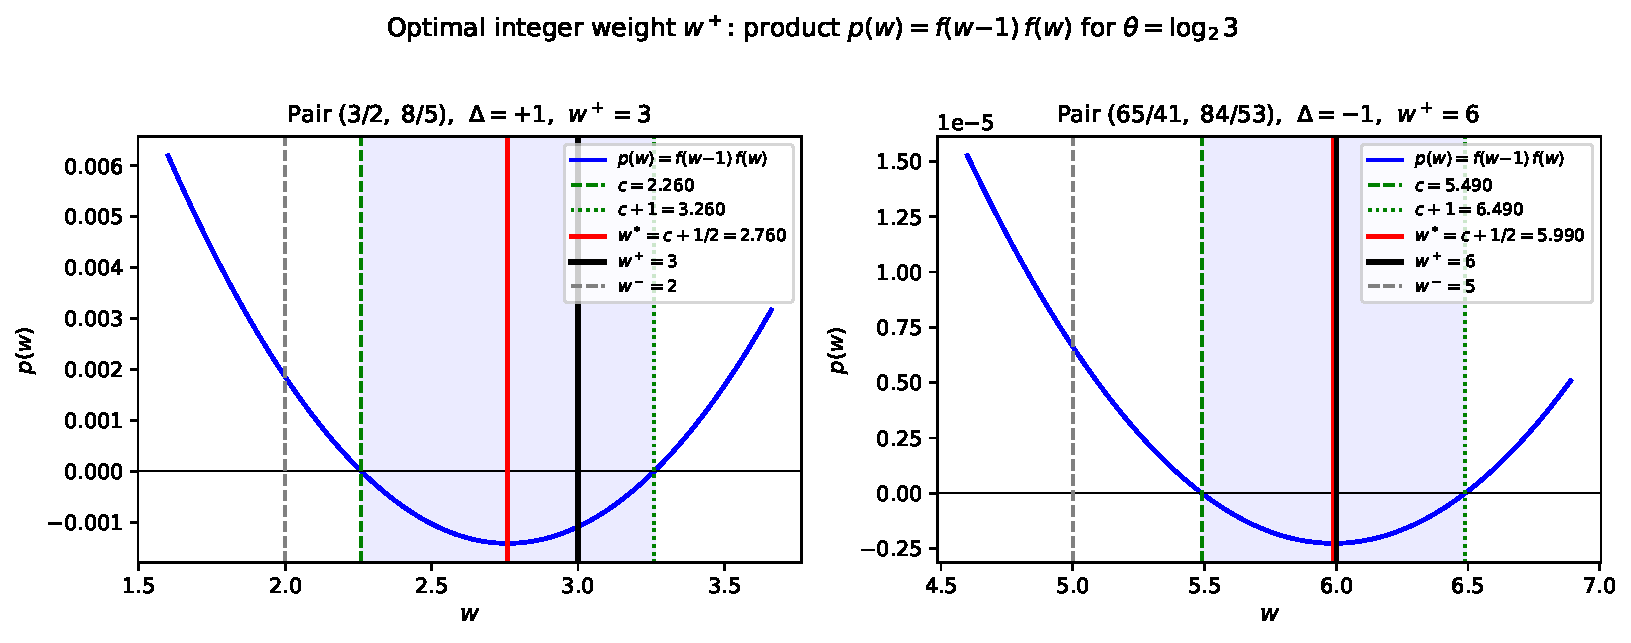
\includegraphics[width=0.95\textwidth]{fig-optimal-weight}
\caption{The product $p(w) = f(w-1)\,f(w)$ for two pairs from the mediant tree for
$\theta = \log_2 3$, illustrating the optimal integer weight $\wplus$.
\emph{Left:} pair $(3/2,\, 8/5)$ with $\Delta = +1$, $c \approx 2.260$, and $\wplus = 3$.
\emph{Right:} pair $(65/41,\, 84/53)$ with $\Delta = -1$, $c \approx 5.490$, and $\wplus = 6$.
In each case the roots of $p$ are at $c$ (where $f(w)=0$, green dashed) and $c+1$
(where $f(w-1)=0$, green dotted); the continuous stationary point $w^* = c + \tfrac{1}{2}$ (red)
is their midpoint; the unique integer in the shaded interval $(c,\,c+1)$ is $\wplus$ (black);
and its companion $\wminus = \wplus - 1$ (grey dashed) lies just outside the interval on the left.
Together $\wminus$ and $\wplus$ are the two weights whose mediants bracket $\theta$.
The two panels illustrate both signs of $\Delta$.}
\label{fig:optimal-weight}
\end{figure}

\paragraph{Algorithm.}
The iteration proceeds as follows.
\begin{enumerate}
  \item Start with an initial bounded pair $(r_0, r_1)$ for $\theta$.
  \item Compute $\Dval$ and $\Kval$.
  \item If $\Kval = 0$, terminate.
  \item Compute $\wplus = \lfloor \Dval/\Kval - o_{2d}/o_{2d+1} \rfloor + 1$ and set $\wminus = \wplus - 1$.
  \item Form the new bounded pair $(\mathrm{Mediant}(r_{2d}, r_{2d+1}, \wminus),\, \mathrm{Mediant}(r_{2d}, r_{2d+1}, \wplus))$ and repeat from step~2.
\end{enumerate}
Because $o_{2d+1}$ grows monotonically along the iteration, $|\varepsilon|$ shrinks
and the iteration converges to $\theta$ (Corollary~\ref{cor:convergence}).

%------------------------------------------------------------
\section{Mediant Words and the Mediant Tree}
\label{sec:parity}
%------------------------------------------------------------

The mediant construction admits a compact combinatorial encoding.
Every estimate produced by the algorithm is either a \emph{leaf} or a \emph{branch},
and the recursive structure of all estimates defines a binary tree whose nodes carry
both rational values and combinatorial words over $\{\OO, \EE\}$.

%------------------------------------------------------------
\subsection{Leaf words}
\label{sec:parity-leaf}
%------------------------------------------------------------

\begin{definition}[Leaf mediant word]
\label{def:parity-alphabet}
Let $\{\OO, \EE\}^*$ denote the set of finite strings over the two-letter alphabet
$\{\OO, \EE\}$.
A \emph{leaf} estimate has denominator $o = 1$, i.e.\ it is a base estimate $e/1$
for some positive integer $e$.
Its \emph{mediant word} is
\[
  \pi(e/1) = \underbrace{\EE \cdots \EE}_{e} \OO,
\]
a string of $e$ copies of $\EE$ followed by one $\OO$.
\end{definition}

The two leaf estimates that initialise the algorithm are $\lfloor\theta\rfloor/1$
and $\lceil\theta\rceil/1$, ordered as $(r_0, r_1)$ so that $r_1$ is the better estimate
(i.e.\ $|\eps_{r_1}| < |\eps_{r_0}|$).
Their mediant words are $\EE^{\lfloor\theta\rfloor}\OO$ and $\EE^{\lceil\theta\rceil}\OO$
respectively.
Since $\theta$ is irrational, $\lceil\theta\rceil = \lfloor\theta\rfloor + 1$, so
$\pi(r_0)$ and $\pi(r_1)$ differ by exactly one $\EE$.
Each word $\EE^k\OO$ contains exactly one $\OO$, so it is not a power of a shorter
word; both $\pi(r_0)$ and $\pi(r_1)$ are therefore primitive.
Moreover, $\EE^k\OO$ is the lower Christoffel word $\mathrm{Ch}^-(k, 1)$
(Definition~\ref{def:christoffel}): its $\OO$ appears at position $k$, matching
the Christoffel formula.
Thus both leaf words are lower Christoffel words of their respective fractions.

%------------------------------------------------------------
\subsection{Branch words and the weighted operators}
\label{sec:parity-branch}
%------------------------------------------------------------

Each branch step produces two new mediant words from the current pair
$(u, v) = (\pi(r_{2d}), \pi(r_{2d+1}))$ by concatenation:

\begin{definition}[Branch mediant word]
\label{def:parity-sequence}
A \emph{branch} estimate $r_{2d+2}$ or $r_{2d+3}$ has two \emph{ordered parents}
$(r_{2d}, r_{2d+1})$ and a positive integer \emph{weight} $w$.
Estimates are indexed so that $r_{2d}$ and $r_{2d+1}$ form the bounded pair at depth
$d$, with $r_{2d+1}$ always the better estimate (smaller $|\eps|$).
The optimal weight $\wplus$ computed from $(r_{2d}, r_{2d+1})$ equals $w_{2d+1}$ in this
indexing; the two child estimates $r_{2d+2}$ and $r_{2d+3}$ carry weights $\wminus$ and
$\wplus$ (i.e.\ $w_{2d+2}$ and $w_{2d+3}$ are $\wplus - 1$ and $\wplus$ in some order).
Write $u = \pi(r_{2d})$ and $v = \pi(r_{2d+1})$ for the parent mediant words.

The two branch words at each depth share the same parents and differ only in the
multiplicity of $v$: one estimate uses weight $\wplus$ and the other uses weight $\wminus$.
Which is the better estimate depends on the errors: writing $\epsminus$ and $\epsplus$ for
the errors of the two candidates (Definition~\ref{def:lambda-eps}),
\[
  w_{2d+3} - w_{2d+2} = \begin{cases} +1 & \text{if } |\epsplus| < |\epsminus|, \\ -1 & \text{otherwise.}\end{cases}
\]
In either case $|\pi(r_{2d+3})| - |\pi(r_{2d+2})| = \pm|v|$.

The branch mediant words are:
\begin{itemize}
  \item $\Dval > 0$ ($r_{2d+1}$ is the upper bound, $v$ plays the role of $\EE$):
    \begin{align*}
      \pi(r_{2d+2}) &= v^{w-1} \cdot u, \\
      \pi(r_{2d+3}) &= v^{w} \cdot u.
    \end{align*}
  \item $\Dval < 0$ ($r_{2d+1}$ is the lower bound, $v$ plays the role of $\OO$):
    \begin{align*}
      \pi(r_{2d+2}) &= u \cdot v^{w-1}, \\
      \pi(r_{2d+3}) &= u \cdot v^{w}.
    \end{align*}
\end{itemize}
Which of the two words is the better estimate $r_{2d+3}$ is determined by comparing
$|\epsminus|$ and $|\epsplus|$; the assignment is not fixed in advance.
\end{definition}

\textbf{Concrete example} ($w = 2$, depth-$0$ leaves
$\pi(r_0) = \mathtt{EO}$, $\pi(r_1) = \mathtt{EEO}$, $\Dval > 0$).
Write $\Phi^w(v, u) = (v^w \cdot u,\; v^{w-1} \cdot u)$ for the pair of branch words
at weight $w$ (the $\Dval > 0$ case):
\[
  \Phi^2\bigl(\mathtt{EEO},\, \mathtt{EO}\bigr)
  = \bigl(\mathtt{EEO}^2\,\mathtt{EO},\; \mathtt{EEO}\,\mathtt{EO}\bigr)
  = \bigl(\mathtt{EEOEEOEO},\; \mathtt{EEOEO}\bigr),
\]
so $\pi(r_3) = \mathtt{EEOEEOEO}$ and $\pi(r_2) = \mathtt{EEOEO}$
(the second component of $\Phi^1(\mathtt{EEO}, \mathtt{EO})$, the $w{-}1$ companion pair).

%------------------------------------------------------------
\subsection{Mediant words are Christoffel words}
\label{sec:parity-standard}
%------------------------------------------------------------

A word is \emph{primitive} if it is not a power $x^k$ of a strictly shorter word $x$
(with $k \geq 2$).

\begin{lemma}[Every mediant word is a lower Christoffel word]
\label{lem:branch-standard-pair}
For every estimate $r = (e, o)$ produced by the mediant tree,
$\pi(r) = \mathrm{Ch}^-(e, o)$, the lower Christoffel word at slope $o/(e+o)$.
In particular, $\pi(r)$ is never an upper Christoffel word, since by
Theorem~\ref{thm:parity-ends-O} every mediant word ends in $\OO$, whereas upper
Christoffel words end in $\EE$.
\end{lemma}

\begin{proof}
By structural induction on the mediant tree.

\emph{Base case.} By §\ref{sec:parity-leaf}, $\pi(e/1) = \EE^e\OO = \mathrm{Ch}^-(e, 1)$.

\emph{Inductive step.}
Let $(r_{2d}, r_{2d+1})$ be a bounded pair with $\Delta = e_{2d+1} o_{2d} - e_{2d} o_{2d+1}$.
By induction $\pi(r_{2d}) = \mathrm{Ch}^-(e_{2d}, o_{2d})$ and $\pi(r_{2d+1}) = \mathrm{Ch}^-(e_{2d+1}, o_{2d+1})$,
both lower Christoffel words (ending in $\OO$), with slopes $o_{2d}/L_{2d}$ and $o_{2d+1}/L_{2d+1}$
(where $L_k = e_k + o_k$) on opposite sides of $\alpha = 1/(1+\theta)$.

When $\Delta > 0$: $r_{2d+1}$ is the upper estimate so $e_{2d+1}/o_{2d+1} > \theta$,
giving $o_{2d+1}/L_{2d+1} < \alpha < o_{2d}/L_{2d}$.
The new word is $v^w u = \pi(r_{2d+1})^w \cdot \pi(r_{2d})$: the smaller-slope word
$\pi(r_{2d+1})$ repeated $w$ times, followed by $\pi(r_{2d})$ once.
By Theorem~\ref{thm:christoffel-concat} (with $e_0 = e_{2d+1}$, $e_1 = e_{2d}$)
this equals $\mathrm{Ch}^-(w\,e_{2d+1} + e_{2d},\; w\,o_{2d+1} + o_{2d})$.

When $\Delta < 0$: $r_{2d+1}$ is the lower estimate so $e_{2d+1}/o_{2d+1} < \theta$,
giving $o_{2d}/L_{2d} < \alpha < o_{2d+1}/L_{2d+1}$.
Thus $\pi(r_{2d})$ has the smaller slope and $\pi(r_{2d+1})$ has the larger slope.
The new word is $u v^w = \pi(r_{2d}) \cdot \pi(r_{2d+1})^w$: the single smaller-slope
word followed by the larger-slope word repeated $w$ times.
By Theorem~\ref{thm:christoffel-concat} (with $e_0 = e_{2d}$, $e_1 = e_{2d+1}$,
$o_0/L_0 < o_1/L_1$, Berstel~\cite{berstel2009} Theorem~1.5.1) this equals
$\mathrm{Ch}^-(e_{2d} + w\,e_{2d+1},\; o_{2d} + w\,o_{2d+1})$.

In both cases $\gcd(e_{2d} + w e_{2d+1},\; o_{2d} + w o_{2d+1}) = 1$ by the Farey adjacency
condition $|e_{2d+1} o_{2d} - e_{2d} o_{2d+1}| = 1$, confirming the result is a valid
lower Christoffel word.
\end{proof}

The Christoffel identification is the key fact connecting the mediant algorithm
to the combinatorics of Sturmian words.
The recurrence $\pi(r_{2d+3}) = v^w \cdot u$ (or $u \cdot v^w$) matches the
standard sequence generation rule for Sturmian words
(Widmer~\cite{widmer2010}, Proposition~2.4.6), with weight $w$ encoding the
partial quotient at that depth.

\begin{remark}
The Christoffel tree --- the binary tree whose nodes are lower Christoffel words
under the same concatenation rules --- is a classical object (Berstel et
al.~\cite{berstel2009}, Chapter~2).
Lemma~\ref{lem:branch-standard-pair} says that the mediant algorithm traverses
exactly this tree: every estimate produced is a node of the Christoffel tree, and
the branch rule is the Christoffel concatenation.
The novelty is not the tree itself but the \emph{driving criterion}: the optimal
weight $\wplus$ (Theorem~\ref{thm:optimal-w}) selects the unique child that
straddles $\theta$, making the traversal goal-directed rather than exhaustive.
\end{remark}

%------------------------------------------------------------
\subsection{The mediant tree}
\label{sec:tree}
%------------------------------------------------------------

The mediant tree is the practical device for generating mediant words of arbitrary
length and precision.
Given a target $\theta$ and a desired precision, one runs the algorithm until the
bounded pair $(r_{2d}, r_{2d+1})$ achieves the required length $e_{2d+1} + o_{2d+1}$.
The mediant word $\pi(r_{2d+1})$ is then read off the tree by the recursive rule:
an interior node $\mathrm{Mediant}(r_0, r_1, w)$ with $\Delta > 0$ yields
$\pi(r_1)^w \cdot \pi(r_0)$, and with $\Delta < 0$ yields
$\pi(r_0) \cdot \pi(r_1)^w$.
Deeper trees produce longer prefixes of the Sturmian word with slope $1/(\theta+1)$
(Section~\ref{sec:sturmian}).

\begin{definition}[Mediant tree]
\label{def:mediant-tree}
The \emph{mediant tree} of an estimate $r$ is defined recursively:
\begin{itemize}
  \item If $r \in \{\lfloor \theta \rfloor, \lceil \theta \rceil\}$, then $r$ is a
        \emph{leaf node}.
  \item Otherwise $r$ is an \emph{interior node} $\mathrm{Mediant}(r_0,\, r_1,\, w)$
        with left subtree $r_0$, right subtree $r_1$, and integer weight $w \geq 0$,
        representing the rational
        \[
          r = \frac{e_0 + w\,e_1}{o_0 + w\,o_1}.
        \]
\end{itemize}
\end{definition}

The two leaves are the unique consecutive integers bracketing $\theta$,
forming the initial bounded pair $(r_0, r_1)$, ordered so that $r_1$ is the better estimate
(i.e.\ $|\varepsilon_{r_1}| < |\varepsilon_{r_0}|$).
Each bounded pair $(r_{2d}, r_{2d+1})$ in the algorithm's sequence consists of two
mediant trees sharing the same leaves; as the iteration advances the trees grow deeper,
recording the full construction history of each estimate.

A detailed worked example for $\theta = \log_2 3$, tracing the first four steps of the
algorithm and the corresponding mediant word decompositions, is given in
Appendix~\ref{app:examples}.

%------------------------------------------------------------
\subsection{The mediant word encodes the fraction}
\label{sec:parity-encoding}
%------------------------------------------------------------

By Lemma~\ref{lem:branch-standard-pair}, the mediant word $\pi(r)$ of an estimate
$r = e/o$ is uniquely determined by its fraction: $\pi(r) = \mathrm{Ch}^-(e, o)$.
The fraction $e/o$ records the full construction history of $r$ via the Euclidean
structure of the mediant algorithm.
Conversely, the fraction $e/o$ can be read off from $\pi(r)$ by counting $\EE$'s and
$\OO$'s.
As the iteration advances, the ratio of $\EE$'s to $\OO$'s in $\pi(r_{2d+1})$ converges to
$\theta$, with strict improvement guaranteed across iterations
(Theorem~\ref{thm:convergence}) but not within a single layer.

%------------------------------------------------------------
\section{Convergence Analysis}
\label{sec:convergence}
%------------------------------------------------------------

\begin{theorem}[Strict decrease of $|\eps|$]
\label{thm:convergence}
At each iteration of the algorithm, $|\eps_{2d+1}|$ strictly decreases.
\end{theorem}

\begin{proof}
By Theorem~\ref{thm:mediant-convergence}, $|\epsplus| < |\eps_{2d+1}|$.
The next iterate assigns the better of $\rminus$ and $\rplus$ as $r_{2d+3}$, so
$|\eps_{2d+3}| \leq |\epsplus| < |\eps_{2d+1}|$.
\end{proof}

\begin{corollary}[Convergence to $\theta$]
\label{cor:convergence}
The sequence of better estimates produced by the algorithm satisfies $\eps_{2d+1} \to 0$.
\end{corollary}

\begin{proof}
From the proof of Corollary~\ref{cor:children-bounded-pair}, writing $f(w) = A + wB$ for
the linear error function and $\odenp, \odenm$ for the two child denominators:
\[
  |f(\wminus)|\,\odenp + |f(\wplus)|\,\odenm = |\Dval| = 1.
\]
Since $f(w) = e_w - \theta\,o_w$ and $\eps_w = f(w)/(\theta\,o_w)$, substituting
$|f(w)| = |\eps_w|\,\theta\,o_w$ gives
\[
  \bigl(|\epsminus| + |\epsplus|\bigr)\,\theta\,\odenm\,\odenp = 1,
\]
so in particular the better child satisfies
\[
  |\eps_{\mathrm{better}}| \leq \frac{1}{2\,\theta\,\odenm\,\odenp}.
\]
(When $\wminus = \wplus - 1 = 0$, the companion $\rminus$ equals the parent $r_{2d}$,
which already satisfies $|\eps_{2d}| > |\eps_{2d+1}|$; the better child is then
$\rplus$, and the bound $|\epsplus| \leq 1/(2\theta\,\odenp)$ still holds.)
Since $\odenp = o_{2d} + \wplus\,o_{2d+1} \geq o_{2d} + o_{2d+1} > o_{2d+1}$, the
denominator of the better child strictly exceeds $o_{2d+1}$; by induction the
denominators diverge.
Since $|\eps_{\mathrm{better}}| \leq 1/(2\,\theta\,\odenm\,\odenp)$ and
$\odenp \to \infty$, we have $\eps_{2d+1} \to 0$.
\end{proof}

\subsection*{Connection to continued fractions}

The connection between the mediant algorithm and continued fractions is a direct
consequence of the Sturmian identity (Theorem~\ref{prop:sturmian}).
In combinatorics on words, the standard sequence for a Sturmian word with slope
$\alpha = 1/(1+\theta)$ is generated by the recurrence $s_n = s_{n-1}^{d_n} \cdot s_{n-2}$,
where the weights $d_n$ are precisely the partial quotients of the continued-fraction
expansion of $\alpha$ (Lothaire~\cite{lothaire2002}, Theorem~2.3.5; Widmer~\cite{widmer2010},
Proposition~2.4.6).
The mediant word sequence agrees with this standard sequence at all interior positions
(Theorem~\ref{prop:sturmian}).
This does \emph{not} imply that the algorithm's weights $\wplus$ equal the partial quotients
$a_k$: the Sturmian identity constrains only interior positions of the words, not which
weights the algorithm selects.
What does follow is that the two children at weights $\wminus$ and $\wplus$ always have
denominators $o_{2d} + \wminus \cdot o_{2d+1}$ and $o_{2d} + \wplus \cdot o_{2d+1}$
(one even-indexed, one odd-indexed depending on which is the better estimate),
mirroring the structure of the classical recurrence $q_{k+1} = a_k q_k + q_{k-1}$.
Whether this implies superlinear denominator growth remains open.

The MT fractions are not in general the same as the CF convergents.
The standard CF recurrence jumps by the full partial quotient $a_k$ at each step,
landing on a new convergent $p_k/q_k$.
The MT algorithm picks the optimal bracketing weight $\wplus$, which may be strictly
less than $a_k$: in that case the new estimate is a \emph{semi-convergent} --- a
Stern-Brocot fraction between two consecutive CF convergents --- not a CF convergent
itself.
Conversely, when $\wplus$ is large it can jump past several intermediate semi-convergents
in one step, skipping CF convergents that lie between them.
Neither sequence is a subsequence of the other: the MT visits some semi-convergents
that CF skips, and CF visits some convergents that the MT skips.
The two sequences are related via the shared Sturmian word structure, but they traverse
different fractions.

%------------------------------------------------------------
%------------------------------------------------------------
\section{Examples and Computational Results}
\label{sec:examples}
%------------------------------------------------------------

Extended tables illustrating the algorithm on $\theta = \log_2 3$ and $\theta = \pi$
are given in Appendix~\ref{app:examples}.


%------------------------------------------------------------
\section{Relationship to Sturmian Sequences}
\label{sec:sturmian}
%------------------------------------------------------------

A \emph{Sturmian word} over $\{\OO, \EE\}$ with slope $\alpha \in (0,1)$ is defined
by
\[
  s_n = \lfloor (n+1)\alpha \rfloor - \lfloor n\alpha \rfloor, \qquad n \geq 0,
\]
encoding the sequence as $\OO$ when $s_n = 1$ and $\EE$ when $s_n = 0$
(see also Section~\ref{sec:background-sturmian}).
Since $\alpha < 1$, we have $s_0 = \lfloor\alpha\rfloor = 0$, so the Sturmian word
always begins with $\EE$.

\subsection{Structural properties of mediant words}

Before stating the main Sturmian identity we record four structural results
about finite mediant words.

\begin{theorem}[Every mediant word ends in $\OO$]
\label{thm:parity-ends-O}
For every estimate $r$ produced by the mediant tree, the mediant word $\pi(r)$
ends in $\OO$.
\end{theorem}

\begin{proof}
By structural induction on the mediant tree.

\emph{Base case.} $\pi(e/1) = \EE^e\OO$, which ends in $\OO$.

\emph{Inductive step.} Assume $\pi(r_0)$ and $\pi(r_1)$ both end in $\OO$.
If $\Delta > 0$ then $\pi(r_{\mathrm{new}}) = \pi(r_1)^w \cdot \pi(r_0)$,
whose last symbol is the last symbol of $\pi(r_0)$, which is $\OO$ by hypothesis.
If $\Delta < 0$ then $\pi(r_{\mathrm{new}}) = \pi(r_0) \cdot \pi(r_1)^w$,
whose last symbol is the last symbol of the final copy of $\pi(r_1)$, again $\OO$.
\end{proof}

\begin{theorem}[Overestimate criterion]
\label{thm:last-sturmian}
Let $\theta > 1$ be irrational, let $r = (e, o)$ be a good estimate of $\theta$
(Definition~\ref{def:good-estimate}), and set $L = e + o$.
Let $s$ be the Sturmian word with slope $\alpha = 1/(1+\theta)$.

\textup{(1)} The Sturmian symbol $s_{L-1}$ satisfies
\[
  s_{L-1} = \begin{cases} \OO & \text{if } e > \theta o \text{ ($r$ an overestimate),} \\
                           \EE & \text{if } e < \theta o \text{ ($r$ an underestimate).} \end{cases}
\]

\textup{(2)} If moreover $r$ is produced by the mediant tree, then
$\pi(r)[-1] = \OO$ (Theorem~\ref{thm:parity-ends-O}), and therefore
$\pi(r)[-1] = s_{L-1}$ if and only if $r$ is an overestimate.
\end{theorem}

\begin{proof}
\textbf{Part (1).}
The Sturmian word satisfies $s_j = \OO$ iff the fractional part
$f_j := \{(j+1)\alpha\}$ lies in $[0, \alpha)$.
So $s_{L-1} = \OO$ iff $\{(e+o)\alpha\} \in [0,\alpha)$.

Set $\Kval = o(e - \theta o)$, so $e = \theta o + \Kval/o$.
Since $\alpha = 1/(1+\theta)$:
\[
  (e+o)\alpha = o + \frac{\Kval\alpha}{o}.
\]
Since $o$ is a positive integer, $\{(e+o)\alpha\} = \{\Kval\alpha/o\}$.
Since $r$ is a good estimate, $|\Kval|/o < 1$; with $\alpha < 1/2$ we have
$|\Kval\alpha/o| < \alpha < 1/2$, so:
\begin{itemize}
  \item $\Kval > 0$: $\{\Kval\alpha/o\} = \Kval\alpha/o \in (0,\alpha)$, so $s_{L-1} = \OO$.
  \item $\Kval < 0$: $\{\Kval\alpha/o\} = 1 + \Kval\alpha/o \in (1-\alpha,1) \subset (\alpha,1)$,
        so $s_{L-1} = \EE$.
\end{itemize}

\textbf{Part (2).}
For a tree estimate, $\pi(r)[-1] = \OO$ by Theorem~\ref{thm:parity-ends-O}.
Combined with Part~(1), $\pi(r)[-1] = s_{L-1}$ iff both equal $\OO$, i.e.\ iff $r$ is an overestimate.
\end{proof}

\begin{remark}
When $r = \mathrm{Mediant}(r_{2d}, r_{2d+1}, \wplus)$ is the child at the bracketing weight,
the overestimate condition $e > \theta o$ is equivalent to $\Dval(r_{2d}, r_{2d+1}) > 0$: since
$\wplus$ is the bracketing weight, $\operatorname{sgn}(e - \theta o) = \operatorname{sgn}(f(\wplus)) = \operatorname{sgn}(B) = \operatorname{sgn}(\Dval)$
(where $f(t) = A + tB$ as in the proof of Theorem~\ref{thm:optimal-w}, and $\Dval = \Dval(r_{2d}, r_{2d+1})$
is the determinant of the \emph{parent pair}).
For the companion child $r = \mathrm{Mediant}(r_{2d}, r_{2d+1}, \wminus)$
(when $\wplus = 1$, the companion is $r_{2d}$ itself), the relationship is reversed.
The sign of $\Dval$ of the parent pair is therefore not a uniform criterion for a general good estimate;
the sign of $\Kval = o(e - \theta o)$ is.
\end{remark}

\begin{theorem}[Universal $\EE\EE$ prefix]
\label{prop:EE-prefix}
For every non-leaf estimate $r$ produced by the mediant tree (i.e.\ $|\pi(r)| > \lceil\theta\rceil + 1$),
the mediant word begins $\pi(r)[0{:}2] = \EE\EE$.
\end{theorem}

\begin{proof}
By Lemma~\ref{lem:branch-standard-pair}, $\pi(r) = \mathrm{Ch}^-(e, o)$.
Every non-leaf estimate $r = e/o$ lies strictly between the two leaf estimates
$\lfloor\theta\rfloor/1$ and $\lceil\theta\rceil/1$, so in particular $e/o > \lfloor\theta\rfloor \geq 1$,
giving $e > o$.
By Definition~\ref{def:christoffel}, $\mathrm{Ch}^-(e,o)[i] = \OO$ iff
$\lfloor(i+1)o/(e+o)\rfloor > \lfloor i\cdot o/(e+o)\rfloor$.
For $i = 0$: $1 \cdot o/(e+o) < 1$ (since $o < e+o$), so
$\lfloor o/(e+o)\rfloor = 0 = \lfloor 0\rfloor$, giving $\pi(r)[0] = \EE$.
For $i = 1$: $e > o$ implies $e+o > 2o$, so $2o/(e+o) < 1$, giving
$\lfloor 2o/(e+o)\rfloor = 0$, and $\pi(r)[1] = \EE$.
Hence $\pi(r)[0{:}2] = \EE\EE$.
\end{proof}

\begin{theorem}[Palindrome invariant]
\label{prop:palindrome}
For every estimate $r$ produced by the mediant tree with $L = |\pi(r)| \geq 2$,
the interior slice $\pi(r)[1{:}L{-}1]$ is a palindrome.
\end{theorem}

\begin{proof}
By Lemma~\ref{lem:branch-standard-pair}, $\pi(r) = \mathrm{Ch}^-(e, o)$ with $L = e+o$.
By Definition~\ref{def:christoffel}, $\mathrm{Ch}^-(e,o) = \EE \cdot U \cdot \OO$ where
$U$ is the palindromic interior (Berstel~\cite{berstel2009}, Chapter~1).
Therefore $\pi(r)[1{:}L{-}1] = U$ is a palindrome.
\end{proof}

\begin{theorem}[Sturmian identity]
\label{prop:sturmian}
Let $\theta > 1$ be irrational, $\alpha = 1/(\theta+1)$, and let $s$ be the Sturmian
sequence with slope $\alpha$.
For every estimate $r$ produced by the mediant tree, with mediant word $\pi(r)$ of
length $N$,
\[
  \pi(r)[i] = s_i \qquad \text{for all } 0 \leq i \leq N-2.
\]
The terminal position $i = N-1$ is excluded: by Theorem~\ref{thm:parity-ends-O}
the mediant always emits $\OO$ there, while by Theorem~\ref{thm:last-sturmian}
the Sturmian emits $\OO$ if $r$ is an overestimate and $\EE$ if $r$ is an underestimate.
\end{theorem}

\begin{proof}
By Lemma~\ref{lem:branch-standard-pair}, $\pi(r) = \mathrm{Ch}^-(e, o)$ with $L = e+o$.
By Definition~\ref{def:christoffel}, $\mathrm{Ch}^-(e,o)[i] = \OO$ iff
$\lfloor(i+1)o/L\rfloor > \lfloor i \cdot o/L\rfloor$, and the Sturmian word
satisfies $s_i = \OO$ iff $\lfloor(i+1)\alpha\rfloor > \lfloor i\alpha\rfloor$.
It suffices to show $\lfloor n \cdot o/L \rfloor = \lfloor n\alpha \rfloor$ for
all $1 \leq n \leq L-1$.

The estimate $r = e/o$ belongs to a bounded pair $(r_{2d}, r_{2d+1})$ at some depth $d$,
with the two fractions $\alpha_0 = o_0/L_0$ and $\alpha_1 = o_1/L_1$ (where $L_k = e_k + o_k$)
satisfying $\alpha_0 < \alpha < \alpha_1$ and the Farey adjacency condition
$o_1 L_0 - o_0 L_1 = \pm 1$.
In particular $o/L$ is one of $\alpha_0$ or $\alpha_1$, and $L = L_k$ for the appropriate $k$.

\textbf{Key lemma (Farey gap).}
For $1 \leq n \leq L-1$, no fraction with denominator $< L$ lies strictly between
$\alpha$ and $o/L$.
\emph{Proof:} Suppose $m/n$ with $0 < n < L$ lies strictly between $\alpha$ and $o/L$.
Then $m/n$ lies strictly between $\alpha_0$ and $\alpha_1$.
By the Farey mediant property, any fraction strictly between two Farey-adjacent
fractions $\alpha_0 = o_0/L_0$ and $\alpha_1 = o_1/L_1$ (with $|o_1 L_0 - o_0 L_1| = 1$)
has denominator at least $L_0 + L_1 > L$, contradicting $n < L$.

\textbf{Agreement.}
Since no fraction with denominator $< L$ lies strictly between $\alpha$ and $o/L$,
for each $1 \leq n \leq L-1$ the two values $n\alpha$ and $n \cdot o/L$ lie in the same
unit interval $[m, m+1)$ for some integer $m$, giving $\lfloor n\alpha \rfloor = \lfloor n \cdot o/L \rfloor$.
Hence $\mathrm{Ch}^-(e,o)[i] = s_i$ for $0 \leq i \leq L-2$.

\paragraph{Terminal position.}
The exclusion of $i = L-1$ follows from Theorems~\ref{thm:parity-ends-O}
and~\ref{thm:last-sturmian}: $\pi(r)$ ends in $\OO$, while $s_{L-1} = \OO$ iff
$r$ is an overestimate ($e/o > \theta$).
\end{proof}

\begin{corollary}[Mismatch characterisation]
\label{cor:mismatch}
The mediant word $\pi(r)$ and the Sturmian prefix $s[0{:}L]$ are identical
if and only if $r$ is an overestimate ($e/o > \theta$).
When $r$ is an underestimate ($e/o < \theta$), they agree at every position except
$i = L-1$, where the mediant emits $\OO$ and the Sturmian emits $\EE$.
\end{corollary}

The single terminal discrepancy is an artefact of truncation, not a genuine
disagreement: the mediant sequence closes its last primitive word with $\OO$ at
position $N-1$, whereas the Sturmian word --- which continues indefinitely --- may
still be in the interior of a longer word at that depth.
As the depth increases and $N \to \infty$, both sequences converge to the same
infinite word.

\begin{remark}
The identification of finite approximants of a Sturmian word with lower Christoffel
words is classical (Lothaire~\cite{lothaire2002}, Berstel et al.~\cite{berstel2009}).
The novel content of Theorem~\ref{prop:sturmian} is the proof via the mediant tree,
which gives an explicit construction of these approximants together with a precise
characterisation of the terminal discrepancy (the last-letter criterion,
Theorems~\ref{thm:parity-ends-O} and~\ref{thm:last-sturmian}).
\end{remark}

This has been verified computationally for several irrational values of $\theta$,
including $\sqrt{2}$, $\log_2 3$, $\log_2 5$, $\phi$, and $\pi$.
For $\theta = \log_2 3$ the verification extends to sequences of length up to
$27{,}869{,}189$ symbols: at every depth the two sequences agree everywhere except
possibly the last symbol, where the mediant emits $\OO$ and the Sturmian emits $\EE$.

\begin{remark}[The mediant sequence is the better finite approximation]
At depths where the two sequences differ, the mediant's finite mediant word is a
closer approximation to $\alpha = 1/(\theta+1)$ in terms of running $\OO$-density.
The terminal $\OO$ emitted by the mediant sequence gives a density slightly
\emph{above} $\alpha$, whereas the Sturmian's terminal $\EE$ gives a density
substantially \emph{below} $\alpha$.

This reflects a structural asymmetry in the two methods.
The Sturmian algorithm at position $N-1$ is mid-word in a longer primitive word,
so it emits $\EE$ --- inherently favouring the above-$\theta$ estimate and leaving the
running density below $\alpha$.
The mediant tree, by contrast, explicitly selects at each step the estimate with
smaller $|\varepsilon|$, i.e.\ $r_{2d+1}$, whichever side of $\theta$ it falls on.
Closing the sequence with $\OO$ at that point reflects this selection: it is the
correct terminal for a word whose ratio $e/o$ slightly underestimates $\theta$, nudging
the running density up toward $\alpha$.

For $\theta = \log_2 3$, the improvement at the discrepancy depths is substantial:
at $N = 1719$ the mediant density error is $1.4 \times 10^{-8}$ against the
Sturmian's $5.8 \times 10^{-4}$ --- roughly four orders of magnitude better.
\end{remark}

The $\OO$-density of $\pi(r)$ for an estimate $e/o$ is
\[
  \frac{o}{e+o} = \frac{1}{e/o + 1} \xrightarrow{e/o \to \theta} \frac{1}{\theta+1} = \alpha,
\]
consistent with the Sturmian slope.

\paragraph{Efficiency and lazy generation.}
Although the mediant words are Sturmian, the mediant tree is a far more efficient
way to generate them.
To produce a prefix of $N$ symbols, the naive Sturmian algorithm must evaluate
$s_n = \lfloor(n+1)\alpha\rfloor - \lfloor n\alpha\rfloor$ at each of the $N$
positions, requiring $O(N)$ real-arithmetic operations.

The mediant algorithm instead builds a compressed representation of the same prefix.
Each iteration requires a constant number of real-arithmetic operations to compute
the next bounded pair and weight; after $k$ iterations the tree encodes a Sturmian
prefix of length $N = e_{2d+1} + o_{2d+1}$.
Empirically $N$ grows rapidly with $k$ (see Section~\ref{sec:convergence}), suggesting
$O(\log N)$ real-arithmetic operations suffice to encode a prefix of length $N$,
though a formal proof of this bound remains open.

Once the tree is built, enumerating the $N$ symbols requires \emph{no real
arithmetic at all}: each node specifies an integer weight $w$ and two child words,
and reading off the sequence is a recursive depth-first traversal governed entirely
by integer counts.
No auxiliary memory beyond the call stack is required.

\paragraph{$\OO\OO$-avoidance.}
Since $\theta > 1$ implies $\alpha = 1/(\theta+1) < 1/2$, the Sturmian word
avoids $\OO\OO$: two consecutive $\OO$'s would require
$\lfloor(n+2)\alpha\rfloor - \lfloor n\alpha\rfloor = 2$, but $2\alpha < 1$ makes
this impossible.
The mediant tree gives an independent structural proof: every mediant word ends in
$\OO$ and begins with $\EE$ (since $e \geq 1$; Lemma~\ref{lem:branch-standard-pair} and Definition~\ref{def:christoffel}), so every concatenation
boundary within a branch word $v^w \cdot u$ or $u \cdot v^w$ reads $\cdots\OO\EE\cdots$;
$\OO\OO$ never arises at any boundary, and by induction never arises anywhere.

\begin{remark}
The weights $w_{2d+1}$ are related to the partial quotients of the continued fraction
expansion of $\theta$, though they are not in general identical to them.
A large weight at step $n$ corresponds to a large partial quotient, producing a long
run of one symbol type in the mediant word --- the same phenomenon that gives rise
to the irregular spacing of $\OO$'s and $\EE$'s in an irrational Sturmian word.
Conversely, small weights correspond to small partial quotients, and the mediant
word advances by only a short block at each such step.
\end{remark}

%------------------------------------------------------------
\section{Extension to $0 < \theta < 1$}
\label{sec:extension}
%------------------------------------------------------------

The algorithm of Sections~\ref{sec:mediant}--\ref{sec:parity} requires $\theta > 1$.
We now show how to handle $\theta \in (0, 1)$ by algebraic reduction, in two stages.

If one were content to accept $\OO\OO$ in the mediant word, no special treatment
would be needed: the algorithm and the Sturmian definition extend formally to any
$\theta > 0$, and for $\theta < 1$ the slope $\alpha = 1/(1+\theta) > 1/2$ makes
$\OO\OO$ unavoidable.
The reductions below are motivated by applications (described in~\cite{paper77})
that require $\OO\OO$-free mediant words.
More concretely: for $\theta \in (0,1)$, setting $\theta' = (1-\theta)/\theta$ (when
$\theta < 1/2$) or $\theta' = \theta/(1-\theta)$ (when $\theta > 1/2$) maps $\theta$
to $\theta' > 1$, giving a slope $1/(1+\theta') < 1/2$ and hence an $\OO\OO$-free
sequence; the counts $e$ and $o$ from that sequence then yield a rational approximant
to the original $\theta$.

\subsection{Case $0 < \theta < \tfrac{1}{2}$}

For $\theta \in (0, \tfrac{1}{2})$, define
\[
  \theta' = \frac{1-\theta}{\theta} = \frac{1}{\theta} - 1 > 1.
\]
Run the algorithm on $\theta'$.
A bounded pair $e/o \approx \theta'$ satisfies $e/o \approx (1-\theta)/\theta$, so
\[
  \theta \approx \frac{o}{e + o}.
\]
The approximant to $\theta$ is therefore $o/(e+o)$, with numerator $o$ (the
$\OO$-count of the mediant word) and denominator $e + o$ (its total length).

\paragraph{Mediant word.}
The mediant word for $\theta'$ has $\OO$-density
\[
  \frac{1}{1 + \theta'} = \frac{1}{1 + (1-\theta)/\theta} = \theta,
\]
which is less than $\tfrac{1}{2}$ since $\theta < \tfrac{1}{2}$.
Consequently the $\OO\OO$-avoidance result of Section~\ref{sec:sturmian} applies:
the mediant word for $\theta'$ is $\OO\OO$-free, and its $\OO$-density converges
to $\theta$.

\paragraph{Sturmian identity.}
The Sturmian word with slope $\alpha' = \theta$ is the infinite mediant word
produced by the mediant tree for $\theta'$ (Theorem~\ref{prop:sturmian}).
This Sturmian word encodes $\theta$ directly: the $\OO$-density of any long prefix
approximates $\theta$ with the same precision as the underlying mediant approximation
of $\theta'$.

\subsection{Case $\tfrac{1}{2} < \theta < 1$}

For $\theta \in (\tfrac{1}{2}, 1)$, note that $1 - \theta \in (0, \tfrac{1}{2})$,
so define
\[
  \theta' = \frac{\theta}{1 - \theta} > 1
\]
and run the algorithm on $\theta'$.
A bounded pair $e/o \approx \theta'$ satisfies $e/o \approx \theta/(1-\theta)$, so
\[
  \theta \approx \frac{e}{e + o}.
\]
No modification of the mediant word is required: the sequence for $\theta'$ is used
solely to produce the counts $e$ and $o$, which then yield the approximant $e/(e+o)$
to the original $\theta$.

\paragraph{Mediant word.}
The mediant word for $\theta'$ has $\OO$-density
\[
  \frac{1}{1 + \theta'} = \frac{1}{1 + \theta/(1-\theta)} = 1 - \theta < \tfrac{1}{2},
\]
so it is $\OO\OO$-free and its Sturmian slope is $1 - \theta$.
The sequence encodes $\theta'$; the rational approximant $e/(e+o)$ to $\theta$ is read
off from the $\EE$- and $\OO$-counts of that sequence.

\paragraph{Summary.}
Table~\ref{tab:extension} collects the reductions for all ranges of $\theta$.

\begin{table}[h]
\centering
\caption{Reductions to the $\theta > 1$ algorithm for all ranges of $\theta$ (four non-trivial, three trivial boundary cases)}
\label{tab:extension}
\begin{tabular}{@{}llll@{}}
\toprule
Range of $\theta$ & Reduction $\theta'$ & Approximant to $\theta$ & $\OO$-density \\
\midrule
$\theta > 1$                & $\theta' = \theta$                  & $e/o$       & $1/(1+\theta) < \tfrac{1}{2}$ \\
$0 < \theta < \tfrac{1}{2}$ & $\theta' = (1-\theta)/\theta$       & $o/(e+o)$   & $\theta < \tfrac{1}{2}$ \\
$\tfrac{1}{2} < \theta < 1$ & $\theta' = \theta/(1-\theta)$       & $e/(e+o)$   & $1-\theta < \tfrac{1}{2}$ \\
$\theta < 0$                & $\theta' = -\theta$ (or above)      & negate      & --- \\
\midrule
$\theta = 0$                & trivial: word $\EE$, $o/(o+e) = 0$  & $0/1$       & --- \\
$\theta = \tfrac{1}{2}$     & trivial: word $\EE\OO$, $o/(o+e) = \tfrac{1}{2}$ & $1/2$ & --- \\
$\theta = 1$                & trivial: word $\OO$, $o/(o+e) = 1$  & $1/1$       & --- \\
\bottomrule
\end{tabular}
\end{table}

%------------------------------------------------------------
\section{Conclusion and Open Problems}
\label{sec:conclusion}
%------------------------------------------------------------

We have presented a theory of rational approximation for real numbers based on
bounded pairs and the weighted mediant construction.
The core algorithm applies to $\theta > 1$; all other real numbers are handled by
algebraic reduction (Section~\ref{sec:extension}).

\paragraph{What is new.}
The weighted mediant step is the classical Stern--Brocot step; the novelty is
Theorem~\ref{thm:optimal-w}, which identifies the \emph{unique optimal weight}
$\wplus$ via a sign-change bracket on the linear error function, giving a closed-form
formula and guaranteeing that each iterate is at least a Stern--Brocot semi-convergent ---
the best approximant achievable in one step from the current bounded pair.
Lemma~\ref{lem:branch-standard-pair} (every mediant word is a lower Christoffel word)
follows from the standard Christoffel concatenation theorem (Berstel et
al.~\cite{berstel2009}); the contribution is the identification that the mediant
algorithm \emph{naturally} produces lower Christoffel words, without any explicit
reference to the Christoffel tree.
The Sturmian identity (Theorem~\ref{prop:sturmian}) and the palindrome invariant
(Theorem~\ref{prop:palindrome}) are consequences of the Christoffel word theory
(Lothaire~\cite{lothaire2002}, Berstel et al.~\cite{berstel2009}); the contribution
is a direct proof via the mediant construction, together with the last-letter criterion
(Theorems~\ref{thm:parity-ends-O} and~\ref{thm:last-sturmian}) which is new.
The mediant tree taken as a whole is a \emph{compressed transducer}: it encodes the
construction history of a length-$N$ Sturmian prefix in $O(\log N)$ integer-arithmetic
steps (empirically; a formal bound remains open), after which the symbols are
enumerated by a purely integer recursive traversal.

\paragraph{Open problems.}
\begin{enumerate}
  \item \textbf{Superlinear denominator growth.}
    Prove that $o_{2d+1}$ grows superlinearly (or exponentially) with the iteration
    count.
    The empirical evidence is strong --- every tested irrational shows at least $4\times$
    growth per two steps --- but a formal proof is lacking.
  \item \textbf{Characterisation of the MT fractions.}
    Every MT fraction is at least a Stern--Brocot semi-convergent; the MT visits
    the subsequence of those whose consecutive mediants straddle $\theta$.
    Characterise this subsequence in terms of the continued-fraction expansion of
    $\theta$, and determine when an MT fraction equals a CF convergent.
  \item \textbf{Cost comparison with CF.}
    The CF algorithm produces convergents in $O(\log N)$ arithmetic steps; the MT does
    likewise but visits different fractions.
    Give a precise comparison of the approximation quality per step between the two
    algorithms.
\end{enumerate}


\begin{thebibliography}{9}
\bibitem{morse1940}
  M.~Morse and G.~A.~Hedlund,
  \textit{Symbolic dynamics II: Sturmian trajectories},
  American Journal of Mathematics \textbf{62} (1940), 1--42.

\bibitem{gkp1994}
  R.~L.~Graham, D.~E.~Knuth, and O.~Patashnik,
  \textit{Concrete Mathematics: A Foundation for Computer Science},
  second edition, Addison-Wesley, 1994.

\bibitem{lothaire2002}
  M.~Lothaire,
  \textit{Algebraic Combinatorics on Words},
  Encyclopedia of Mathematics and its Applications \textbf{90},
  Cambridge University Press, 2002.

\bibitem{widmer2010}
  S.~Widmer,
  \textit{Topics in Word Complexity},
  PhD thesis, Universit\'e Claude Bernard Lyon~1, 2010.
  HAL: \texttt{tel-00812583}.

\bibitem{berstel2009}
  J.~Berstel, A.~Lauve, C.~Reutenauer, and F.~Saliola,
  \textit{Combinatorics on Words: Christoffel Words and Repetitions in Words},
  CRM Monograph Series \textbf{27},
  American Mathematical Society, Providence, RI, 2009.

\bibitem{paper77}
  J.~Seymour,
  \textit{Mediants and Collatz: Constructing Generalised Collatz Trajectories
  via Rational Approximation},
  \texttt{https://github.com/wildducktheories/collatz}, Paper~77 (2026).

\end{thebibliography}

%============================================================
\appendix
%============================================================

%------------------------------------------------------------
\section{Proof of Theorem~\ref{thm:optimal-w}}
\label{app:optimal-w}
%------------------------------------------------------------

We prove the closed-form formula $\wplus = \lfloor -A/B \rfloor + 1$ directly from
the bracketing condition, using only a linear sign argument.

We have a bounded pair $(r_{2d}, r_{2d+1})$ bracketing $\theta$, with
\[
  A = e_{2d} - \theta\,o_{2d}, \qquad B = e_{2d+1} - \theta\,o_{2d+1}.
\]
Since $r_{2d}$ and $r_{2d+1}$ are on opposite sides of $\theta$ we have $\operatorname{sgn}(A) = -\operatorname{sgn}(B)$,
so $A/B < 0$ and $c := -A/B > 0$.
The two weighted mediants are
\[
  \rminus = \frac{e_{2d} + (w-1)\,e_{2d+1}}{o_{2d} + (w-1)\,o_{2d+1}}, \qquad
  \rplus = \frac{e_{2d} + w\,e_{2d+1}}{o_{2d} + w\,o_{2d+1}},
\]
with signed errors (numerators of $\epsminus$, $\epsplus$ up to positive denominators)
\[
  A + (w-1)B \qquad \text{and} \qquad A + wB.
\]

\paragraph{Bracketing condition.}

The pair $(\rminus, \rplus)$ brackets $\theta$ iff $\epsminus$ and $\epsplus$ have opposite signs,
i.e.\ $(A + (w-1)B)(A + wB) < 0$.
Writing $c = -A/B$, this product equals $B^2\,(w - 1 - c)(w - c)$, which is negative
iff $w - 1 - c$ and $w - c$ have opposite signs, i.e.\
\[
  w - 1 < c < w \qquad \Longleftrightarrow \qquad c - 1 < w - 1 \leq c
  \qquad \Longleftrightarrow \qquad w = \lfloor c \rfloor + 1.
\]
Since $\theta$ is irrational, $A + nB \neq 0$ for all integers $n$, so $c$ is never
an integer and the condition is strict: exactly one integer $w$ satisfies it, namely
\[
  \wplus = \lfloor -A/B \rfloor + 1.
\]
We also write $\wminus = \wplus - 1 = \lfloor -A/B \rfloor$ for the companion weight.

\paragraph{Expression in terms of $\Dval$ and $\Kval$.}

Recall $\Kval = o_{2d+1}B$ and $A\,o_{2d+1} - B\,o_{2d} = -\Dval$, giving
$A = (Bo_{2d} - \Dval)/o_{2d+1}$, so
\[
  \frac{-A}{B} = \frac{\Dval}{o_{2d+1}B} - \frac{o_{2d}}{o_{2d+1}}
               = \frac{\Dval}{\Kval} - \frac{o_{2d}}{o_{2d+1}},
\]
and therefore
\[
  \wplus = \left\lfloor \frac{\Dval}{\Kval} - \frac{o_{2d}}{o_{2d+1}} \right\rfloor + 1,
\]
completing the proof of Theorem~\ref{thm:optimal-w}.

\paragraph{Termination.}
When $\Kval = 0$, $r_{2d+1}$ is an exact rational representation of $\theta$;
no further improvement is possible and the algorithm terminates.

%------------------------------------------------------------
\section{Examples and Computational Results}
\label{app:examples}
%------------------------------------------------------------

\subsection{Worked example: mediant words for \texorpdfstring{$\log_2 3$}{log\_2(3)}}

\begin{example}[Mediant words and trees for $\log_2 3$]
\label{ex:log2-3}
Starting from the initial bounded pair $(r_0, r_1) = (1/1,\, 2/1)$ with
$\theta = \log_2 3 \approx 1.58496$,
the algorithm produces the following sequence of bounded pairs.
At each depth $d$, weight $w_{2d+1}$ is used to compute the two candidates
$\rminus = \mathrm{Mediant}(r_{2d}, r_{2d+1}, w_{2d+1}-1)$ and
$\rplus = \mathrm{Mediant}(r_{2d}, r_{2d+1}, w_{2d+1})$;
the better estimate (smaller $|\eps|$) becomes $r_{2d+3}$.

\medskip
\begin{center}
\begin{tabular}{@{}cllllcll@{}}
\toprule
$d$ & $r_{2d}$ & $r_{2d+1}$ & $\eps_{r_{2d}}$ & $\eps_{r_{2d+1}}$ & $w_{2d+1}$ & $\rminus$ & $\rplus$ \\
\midrule
0 & $1/1$   & $2/1$   & $-0.369$ & $+0.262$ & 2 & $3/2$   & $5/3$   \\
1 & $3/2$   & $5/3$   & $-0.054$ & $+0.052$ & 1 & $3/2$   & $8/5$   \\
2 & $3/2$   & $8/5$   & $-0.054$ & $+0.009$ & 3 & $19/12$ & $27/17$ \\
3 & $27/17$ & $19/12$ & $+0.002$ & $-0.001$ & 3 & $65/41$ & $84/53$ \\
\bottomrule
\end{tabular}
\end{center}
\medskip

The leaf words are $\pi(r_0) = \mathtt{EO}$ and $\pi(r_1) = \mathtt{EEO}$.
Reading the word decomposition bottom-up:

\medskip
\noindent
\textbf{Level 1} ($d=0$, $w_1=2$, $\Delta>0$,
$\pi(r_3)=\pi(r_1)^2\cdot\pi(r_0)$, $\pi(r_2)=\pi(r_1)^1\cdot\pi(r_0)$):
\[
\underbrace{
  \underbrace{\mathtt{EEO}}_{\pi(r_1)}
  \underbrace{\mathtt{EEO}}_{\pi(r_1)}
  \underbrace{\mathtt{EO}}_{\pi(r_0)}
}_{\pi(r_3)=\mathtt{EEOEEOEO}}
\qquad
\underbrace{
  \underbrace{\mathtt{EEO}}_{\pi(r_1)}
  \underbrace{\mathtt{EO}}_{\pi(r_0)}
}_{\pi(r_2)=\mathtt{EEOEO}}
\]

\noindent
\textbf{Level 2} ($d=1$, $w_3=1$, $\Delta>0$,
$\pi(r_5)=\pi(r_3)^1\cdot\pi(r_2)$, $\pi(r_4)=\pi(r_2)$):
\[
\underbrace{
  \underbrace{\mathtt{EEOEEOEO}}_{\pi(r_3)}
  \underbrace{\mathtt{EEOEO}}_{\pi(r_2)}
}_{\pi(r_5)=\mathtt{EEOEEOEOEEOEO}}
\qquad
\underbrace{
  \underbrace{\mathtt{EEOEO}}_{\pi(r_2)}
}_{\pi(r_4)=\mathtt{EEOEO}}
\]

\noindent
\textbf{Level 3} ($d=2$, $w_5=3$, $\Delta>0$,
$\pi(r_7)=\pi(r_5)^2\cdot\pi(r_4)$):
\[
\underbrace{
  \underbrace{\mathtt{EEOEEOEOEEOEO}}_{\pi(r_5)}
  \;
  \underbrace{\mathtt{EEOEEOEOEEOEO}}_{\pi(r_5)}
  \;
  \underbrace{\mathtt{EEOEO}}_{\pi(r_4)}
}_{\pi(r_7)}
\]

The same estimates as mediant trees (depths $d=1$ and $d=2$):
\begin{align*}
  r_{2} = 3/2 &= \mathrm{Mediant}(\underbrace{1}_{\text{leaf}},\;
                   \underbrace{2}_{\text{leaf}},\; w=1), \\
  r_{3} = 5/3 &= \mathrm{Mediant}(\underbrace{1}_{\text{leaf}},\;
                   \underbrace{2}_{\text{leaf}},\; w=2), \\
  r_{4} = 3/2 &= \mathrm{Mediant}(\mathrm{Mediant}(1,\, 2,\, 1),\;
                   \mathrm{Mediant}(1,\, 2,\, 2),\; w=0), \\
  r_{5} = 8/5 &= \mathrm{Mediant}(\mathrm{Mediant}(1,\, 2,\, 1),\;
                   \mathrm{Mediant}(1,\, 2,\, 2),\; w=1).
\end{align*}
A weight of $w=0$ means the left subtree is used directly (contributing zero copies
of the right subtree).
\end{example}

\subsection{Approximating \texorpdfstring{$\log_2 3$}{log\_2(3)}}

Table~\ref{tab:log23} shows 22 steps of the algorithm for $\theta = \log_2 3$,
starting from $r_0 = 1/1$, $r_1 = 2/1$.
Note the large weight $w = 24$ at depth $d=6$ and $w=55$ at depth $d=10$, corresponding
to large partial quotients of the continued fraction of $\log_2 3$, which produce
large jumps in precision.

\begin{table}[ht]
\centering
\caption{Successive bounded pairs approximating $\log_2 3 \approx 1.58496\ldots$}
\label{tab:log23}
\resizebox{\textwidth}{!}{%
\begin{tabular}{@{}clllrcll@{}}
\toprule
$d$ & $r_{2d}$ & $r_{2d+1}$ & $\eps_{r_{2d}}$ & $\eps_{r_{2d+1}}$ & $\wplus$ & $\rminus$ & $\rplus$ \\
\midrule
0  & $1/1$         & $2/1$          & $-0.369$ & $+0.262$ & 2  & $3/2$         & $5/3$         \\
1  & $3/2$         & $5/3$          & $-0.054$ & $+0.052$ & 1  & $3/2$         & $8/5$         \\
2  & $3/2$         & $8/5$          & $-0.054$ & $+0.009$ & 3  & $19/12$       & $27/17$       \\
3  & $27/17$       & $19/12$        & $+0.002$ & $-0.001$ & 3  & $65/41$       & $84/53$       \\
4  & $65/41$       & $84/53$        & $+2.54\times10^{-4}$ & $-3.59\times10^{-5}$ & 6  & $485/306$     & $569/359$     \\
5  & $485/306$     & $569/359$      & $+3.04\times10^{-6}$ & $-2.70\times10^{-6}$ & 1  & $485/306$     & $1054/665$    \\
6  & $485/306$     & $1054/665$     & $+3.04\times10^{-6}$ & $-5.98\times10^{-8}$ & 24 & $24727/15601$ & $25781/16266$ \\
7  & $25781/16266$ & $24727/15601$  & $-1.42\times10^{-9}$ & $+1.06\times10^{-9}$ & 2  & $50508/31867$ & $75235/47468$ \\
8  & $75235/47468$ & $50508/31867$  & $+2.10\times10^{-10}$ & $-2.08\times10^{-10}$ & 2 & $125743/79335$ & $176251/111202$ \\
9  & $125743/79335$ & $176251/111202$ & $+4.20\times10^{-11}$ & $-2.95\times10^{-11}$ & 2 & $301994/190537$ & $478245/301739$ \\
10 & $478245/301739$ & $301994/190537$ & $-1.07\times10^{-11}$ & $+3.08\times10^{-13}$ & 55 & $16785921/10590737$ & $17087915/10781274$ \\
11 & $16785921/10590737$ & $17087915/10781274$ & $-4.50\times10^{-15}$ & $+1.03\times10^{-15}$ & 5 & $85137581/53715833$ & $102225496/64497107$ \\
12 & $102225496/64497107$ & $85137581/53715833$ & $+1.23\times10^{-16}$ & $-5.88\times10^{-17}$ & 3 & $272500658/171928773$ & $357638239/225644606$ \\
13 & $272500658/171928773$ & $357638239/225644606$ & $+9.47\times10^{-18}$ & $-6.79\times10^{-18}$ & 2 & $630138897/397573379$ & $987777136/623217985$ \\
14 & $987777136/623217985$ & $630138897/397573379$ & $-2.30\times10^{-18}$ & $+2.42\times10^{-19}$ & 15 & $9809721694/6189245291$ & $10439860591/6586818670$ \\
15 & $9809721694/6189245291$ & $10439860591/6586818670$ & $-1.41\times10^{-20}$ & $+1.40\times10^{-21}$ & 10 & $103768467013/65470613321$ & $114208327604/72057431991$ \\
16 & $114208327604/72057431991$ & $103768467013/65470613321$ & $+6.96\times10^{-23}$ & $-6.41\times10^{-23}$ & 2 & $217976794617/137528045312$ & $321745261630/202998658633$ \\
17 & $321745261630/202998658633$ & $217976794617/137528045312$ & $-1.67\times10^{-23}$ & $+5.95\times10^{-24}$ & 5 & $1193652440098/753110839881$ & $1411629234715/890638885193$ \\
18 & $1411629234715/890638885193$ & $1193652440098/753110839881$ & $+7.97\times10^{-25}$ & $-1.44\times10^{-25}$ & 7 & $8573543875303/5409303924479$ & $9767196315401/6162414764360$ \\
19 & $8573543875303/5409303924479$ & $9767196315401/6162414764360$ & $+1.11\times10^{-26}$ & $-7.83\times10^{-27}$ & 2 & $18340740190704/11571718688839$ & $28107936506105/17734133453199$ \\
20 & $28107936506105/17734133453199$ & $18340740190704/11571718688839$ & $-2.06\times10^{-27}$ & $+1.01\times10^{-27}$ & 4 & $83130157078217/52449289519716$ & $101470897268921/64021008208555$ \\
21 & $101470897268921/64021008208555$ & $83130157078217/52449289519716$ & $+1.63\times10^{-28}$ & $-2.51\times10^{-29}$ & 8 & $683381996816440/431166034846567$ & $766512153894657/483615324366283$ \\
\bottomrule
\end{tabular}}
\end{table}

\subsection{Approximating \texorpdfstring{$\pi$}{pi}}


Table~\ref{tab:pi} shows 22 steps for $\theta = \pi$, starting from $r_0 = 4/1$,
$r_1 = 3/1$.
The classical approximant $355/113$ appears at depth $d=1$ (as $\rplus$) with
$\eps \approx +8.49 \times 10^{-8}$, and the weight $w=293$ at depth $d=2$
produces an immediate jump of roughly three orders of magnitude
(from $|\varepsilon| \approx 8.49 \times 10^{-8}$ to $|\varepsilon| \approx 1.06 \times 10^{-10}$).

\begin{table}[ht]
\centering
\caption{Successive bounded pairs approximating $\pi \approx 3.14159\ldots$}
\label{tab:pi}
\resizebox{\textwidth}{!}{%
\begin{tabular}{@{}clllrcll@{}}
\toprule
$d$ & $r_{2d}$ & $r_{2d+1}$ & $\eps_{r_{2d}}$ & $\eps_{r_{2d+1}}$ & $\wplus$ & $\rminus$ & $\rplus$ \\
\midrule
0  & $4/1$     & $3/1$     & $+0.273$            & $-0.045$            & 7   & $22/7$         & $25/8$         \\
1  & $25/8$    & $22/7$    & $-5.0\times10^{-3}$ & $+4.02\times10^{-4}$ & 15  & $333/106$      & $355/113$      \\
2  & $333/106$ & $355/113$ & $-2.65\times10^{-5}$ & $+8.49\times10^{-8}$ & 293 & $103993/33102$ & $104348/33215$ \\
3  & $103993/33102$ & $104348/33215$ & $-1.84\times10^{-10}$ & $+1.06\times10^{-10}$ & 2  & $208341/66317$  & $312689/99532$  \\
4  & $208341/66317$  & $312689/99532$  & $-3.89\times10^{-11}$ & $+9.28\times10^{-12}$ & 3  & $833719/265381$  & $1146408/364913$  \\
5  & $833719/265381$  & $1146408/364913$  & $-2.77\times10^{-12}$ & $+5.13\times10^{-13}$ & 4  & $4272943/1360120$  & $5419351/1725033$  \\
6  & $4272943/1360120$  & $5419351/1725033$  & $-1.29\times10^{-13}$ & $+7.05\times10^{-15}$ & 15 & $80143857/25510582$ & $85563208/27235615$ \\
7  & $85563208/27235615$ & $80143857/25510582$ & $+2.74\times10^{-16}$ & $-1.84\times10^{-16}$ & 2  & $165707065/52746197$ & $245850922/78256779$ \\
8  & $165707065/52746197$ & $245850922/78256779$ & $+5.22\times10^{-17}$ & $-2.49\times10^{-17}$ & 2  & $411557987/131002976$ & $657408909/209259755$ \\
9  & $411557987/131002976$ & $657408909/209259755$ & $+6.16\times10^{-18}$ & $-5.45\times10^{-18}$ & 1  & $411557987/131002976$ & $1068966896/340262731$ \\
10 & $411557987/131002976$ & $1068966896/340262731$ & $+6.16\times10^{-18}$ & $-9.77\times10^{-19}$ & 3  & $2549491779/811528438$ & $3618458675/1151791169$ \\
11 & $2549491779/811528438$ & $3618458675/1151791169$ & $+1.76\times10^{-19}$ & $-1.65\times10^{-19}$ & 1  & $2549491779/811528438$ & $6167950454/1963319607$ \\
12 & $2549491779/811528438$ & $6167950454/1963319607$ & $+1.76\times10^{-19}$ & $-2.43\times10^{-20}$ & 3  & $14885392687/4738167652$ & $21053343141/6701487259$ \\
13 & $14885392687/4738167652$ & $21053343141/6701487259$ & $+9.94\times10^{-21}$ & $-8.33\times10^{-23}$ & 85 & $1783366216531/567663097408$ & $1804419559672/574364584667$ \\
14 & $1804419559672/574364584667$ & $1783366216531/567663097408$ & $-5.85\times10^{-25}$ & $+3.91\times10^{-25}$ & 2  & $3587785776203/1142027682075$ & $5371151992734/1709690779483$ \\
15 & $3587785776203/1142027682075$ & $5371151992734/1709690779483$ & $-1.00\times10^{-25}$ & $+6.28\times10^{-26}$ & 2  & $8958937768937/2851718461558$ & $14330089761671/4561409241041$ \\
16 & $14330089761671/4561409241041$ & $8958937768937/2851718461558$ & $+2.20\times10^{-26}$ & $-2.46\times10^{-27}$ & 15 & $139755218526789/44485467702853$ & $148714156295726/47337186164411$ \\
17 & $148714156295726/47337186164411$ & $139755218526789/44485467702853$ & $-9.99\times10^{-29}$ & $+5.13\times10^{-29}$ & 3  & $428224593349304/136308121570117$ & $567979811876093/180793589272970$ \\
18 & $567979811876093/180793589272970$ & $428224593349304/136308121570117$ & $+1.17\times10^{-29}$ & $-1.21\times10^{-30}$ & 13 & $5706674932067741/1816491048114374$ & $6134899525417045/1952799169684491$ \\
19 & $5706674932067741/1816491048114374$ & $6134899525417045/1952799169684491$ & $+7.43\times10^{-32}$ & $-1.55\times10^{-32}$ & 5  & $30246273033735921/9627687726852338$ & $36381172559152966/11580486896536829$ \\
20 & $30246273033735921/9627687726852338$ & $36381172559152966/11580486896536829$ & $+1.45\times10^{-33}$ & $-1.40\times10^{-33}$ & 1  & $30246273033735921/9627687726852338$ & $66627445592888887/21208174623389167$ \\
21 & $30246273033735921/9627687726852338$ & $66627445592888887/21208174623389167$ & $+1.45\times10^{-33}$ & $-1.07\times10^{-34}$ & 7  & $430010946591069243/136876735467187340$ & $496638392183958130/158084910090576507$ \\
\bottomrule
\end{tabular}}
\end{table}

\end{document}
